\documentclass[aspectratio=169]{beamer}
\usepackage[absolute,overlay]{textpos}
\usepackage{tikz}
\usetikzlibrary{shadings}
\usepackage[utf8]{inputenc}
\usepackage{amsmath,amssymb}
\usepackage[russian]{babel}
\usepackage{cancel} %для сокращения слагаемых
\usepackage{wrapfig} % подписи к картинкам
\usepackage{xcolor}
\usepackage{graphicx}
\usepackage{makecell}
\title[]{Лабораторная работа: Численные методы вычисления интегралов}
\author[]{Веселов Фёдор, Ушаков Роман, Босенко Борис, Ежелев Георгий}

\newlength{\RightSidebarWidth} 
\setlength{\RightSidebarWidth}{1cm}

% используем внешний шаблон sidebar
\useoutertheme[right]{sidebar}

% убираем стандартный верхний и нижний колонтитулы
\setbeamertemplate{headline}{}
\setbeamertemplate{footline}{}

% наш вариант правой боковой панели
\setbeamertemplate{sidebar right}{%
	\begin{tikzpicture}[remember picture, overlay]
		% Можно использовать structure.fg напрямую
		\shade[top color=structure.fg!60, bottom color=structure.fg!10]
		([xshift=-2.5cm]current page.north east) rectangle (current page.south east);
		\node[anchor=center, align=center, font=\tiny, text width=2.4cm]
		at ([xshift=-1.2cm, yshift=-1.25cm]current page.north east) {
			\scriptsize \textcolor{structure.fg}{\textbf{Численное интегрирование}}\\
			\tiny Веселов Фёдор\\[0.5em]
			\tiny Ушаков Роман\\[0.5em]
			\tiny Босенко Борис\\[0.5em]
			\tiny Ежелев Георгий\\[0.5em]
		};
	\end{tikzpicture}
}

% чтобы содержимое не залезало под полосу
\setbeamersize{text margin right=\RightSidebarWidth}

\begin{document}
	\begin{frame}
		\titlepage
	\end{frame}
	
	\begin{frame}
		\textcolor{orange}{\large{Видеоматериалы можно найти по ссылке: https://drive.google.com/drive/folders/1EXT7La5MnyfdQ7618N8fT-iFyFJS5yVN}}\\[1cm]
	\end{frame}
	
	\begin{frame}
		\large \textbf{\textcolor{structure.fg}{Индивидуальная часть. Ежелев Георгий}}\\
		\textbf{Дан интеграл функции: } \[\int_{0}^{1}  e^{-x} dx\]\\
		Формула правых прямоугольников:\\
		\[\lim_{n \to \infty}\frac{b-a}{n}*\sum_{i=1}^{n}f(x_i)\]\\
		Разбиение равномерное. Воспользуемся \textcolor{orange}{формулой суммы геометрической прогрессии} и \textcolor{orange}{эквивалентностью} $e^{x} - 1 \sim x$\\
		\[\lim_{n \to \infty} \frac{1}{n} * \sum_{k=1}^{n} e^{-\frac{k}{n}} = \lim_{n \to \infty} \frac{1}{n} * \frac{e^{-\frac{n}{n}} - 1 }{e^{-\frac{1}{n}} - 1} =\]\[= \lim_{n \to \infty} \frac{1}{n} * \frac{e^{-1} - 1 }{e^{-\frac{1}{n}} - 1} = \lim_{n \to \infty} \frac{1}{n} * \frac{e^{-1} - 1}{-\frac{1}{n}} = \lim_{n \to \infty} -(e^{-1} - 1) = \boxed{1 - e^{-1}}\]\\
	\end{frame}
	\begin{frame}
		\large \textbf{\textcolor{structure.fg}{Задание №3 - Проверка существования интеграла}}\\
	\(e^{-x}\) интегрируема на [0,1], т.к. является непрерывной на данном отрезке.\\
	\large \textbf{\textcolor{structure.fg}{Задание №4 - Проверка прямым интегрированием}}\\
	\[\int_{0}^{1}  e^{-x} dx = -e^{-x}\Big\vert_{0}^{1} = \boxed{1 - e^{-1}}\]\\

	\large \textbf{\textcolor{structure.fg}{Часть №2 - численное интегрирование}}\\
	$\bullet$Язык программирования - Python.\\
	$\bullet$Отрисовка графиков по посчитанным точкам - библиотека matplotlib\\
	$\bullet$Значение определенного интеграла: \(I = 1-\frac{1}{e} \approx 0.63212...\)\\
	\end{frame}
	\begin{frame}
		
	\large \textbf{\textcolor{structure.fg}{Метод левых прямоугольников}}\\
	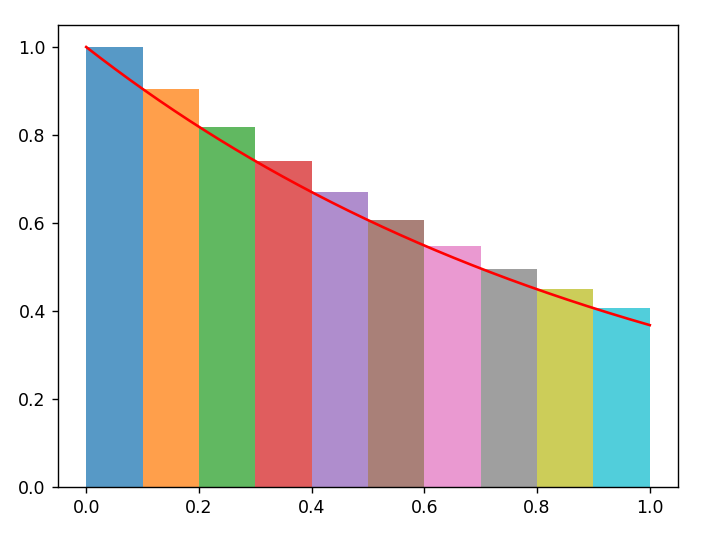
\includegraphics[width = 7.5cm, height = 4cm]{left_10.png}\\
	n = 10. Ранг разбиения 0.1. \\
	\begin{tikzpicture}[remember picture,overlay]
		\node[draw,rounded corners,fill=blue!10,text width=5.5cm,align=left]
		at (10.25,4.5) {Результат: \(R \approx 0.66425\). \\Теор. значение: \(I \approx 0.63212...\)};
	\end{tikzpicture}
	\begin{tikzpicture}[remember picture,overlay]
		\node[draw,rounded corners,fill=green!10,text width=5.5cm,align=left]
		at (10.15,2.5) {Формула погрешности:\[|R_n| \leq \max_{x \in [a, b]} |f^\prime(x)| \frac{(b-a)^2}{2n}\]};
	\end{tikzpicture}

	
	Тогда имеем:
	\(|R_n| \leq \max_{x \in [0, 1]} |-e^{-x}| \frac{1}{2n} = \boxed{\frac{1}{2n}}\)
	
	При n = 10 погрешность \(|R_n| \leq 0.05\), \(|I - R|\approx 0.03213 \leq R_n\) - теоретическая погрешность соблюдена. 
\end{frame}
\begin{frame}
	\large \textbf{\textcolor{structure.fg}{Метод правых прямоугольников}}\\
	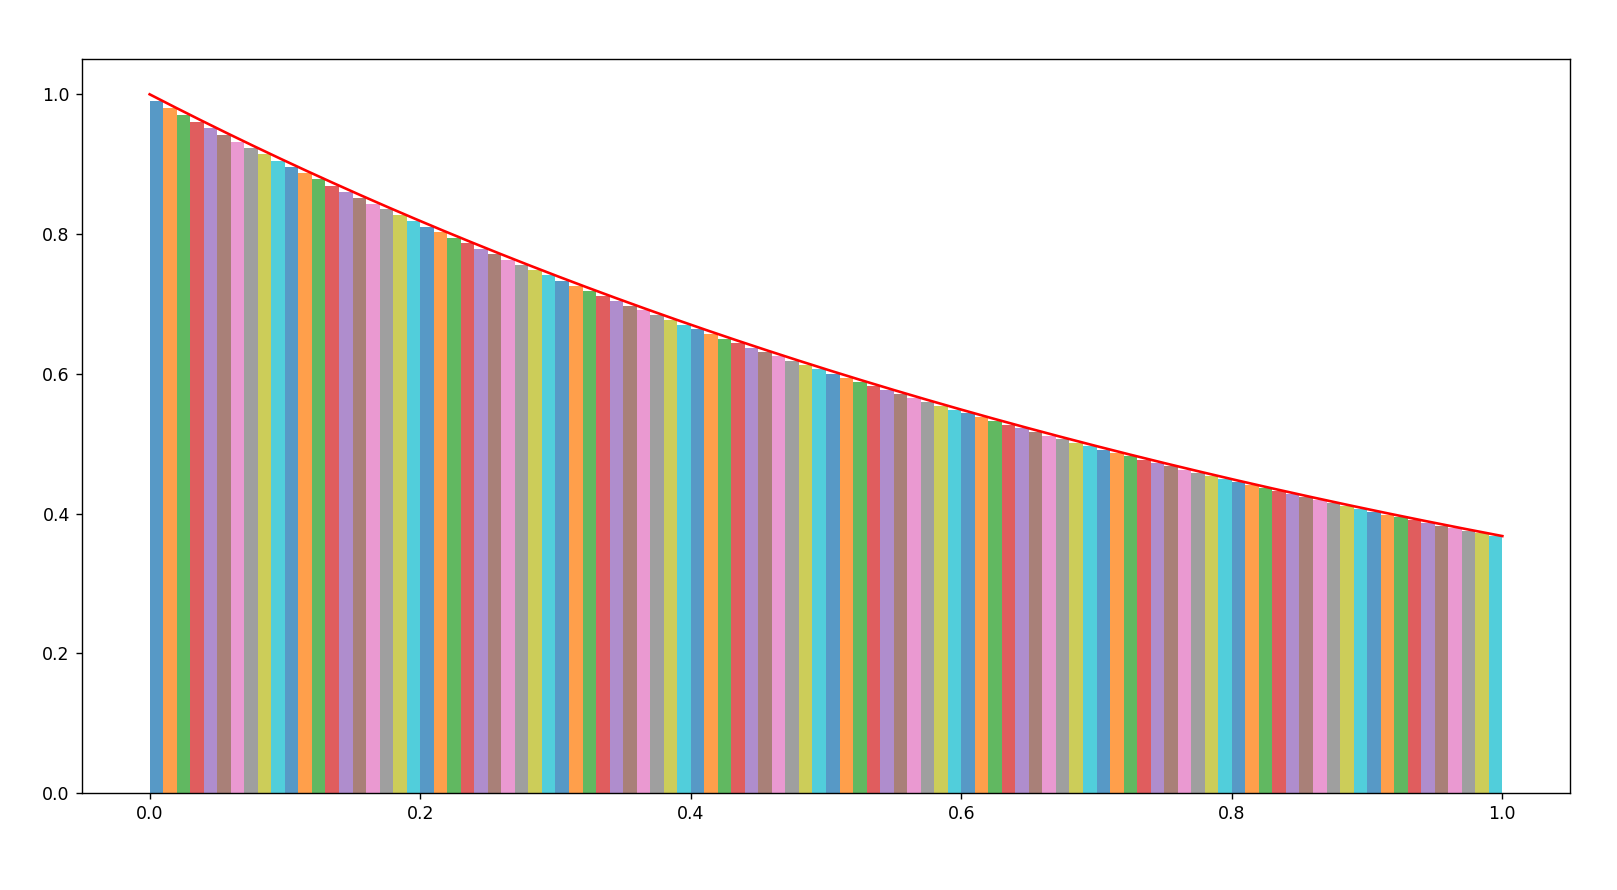
\includegraphics[width = 7.5cm, height = 5cm]{right_100.png}\\
	\begin{tikzpicture}[remember picture,overlay]
		\node[draw,rounded corners,fill=blue!10,text width=5.5cm,align=left]
		at (10.25,4.5) {Результат: \(R \approx 0.62896\),\\ Теор. значение: \(I \approx 0.63212\).};
	\end{tikzpicture}
		\begin{tikzpicture}[remember picture,overlay]
		\node[draw,rounded corners,fill=green!10,text width=5.5cm,align=left]
		at (10.15,2.5) {Формула погрешности:\[|R_n| \leq \max_{x \in [a, b]} |f^\prime(x)| \frac{(b-a)^2}{2n}\]};
	\end{tikzpicture}
	n = 100. Ранг разбиения 0.01. \\
	Формула погрешности та же, что и в предыдущем методе:
	\[|R_n| \leq \frac{1}{2n}\]
	При n = 100 погрешность: \(|R_n| \leq 0.005\), \(|I - R|\approx 0.00316 \leq R_n\) - теоретическая погрешность соблюдена.
	\end{frame}
	\begin{frame}
		\large \textbf{\textcolor{structure.fg}{Метод трапеций}}\\
		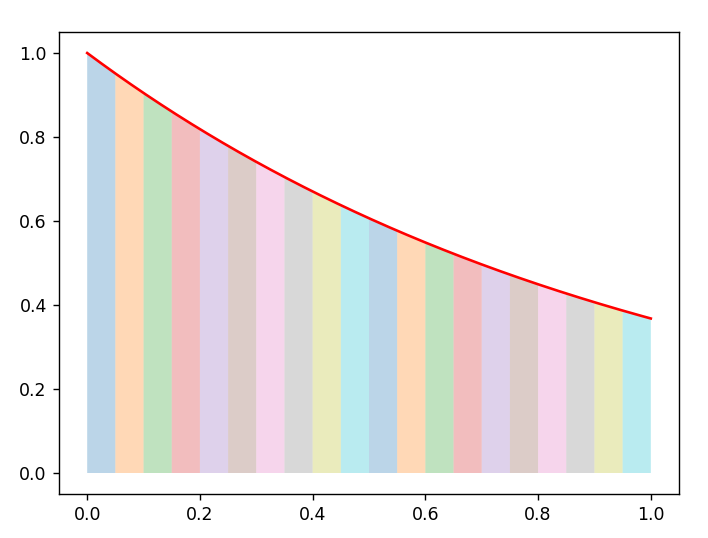
\includegraphics[width = 7.5cm, height = 4cm]{trap_10.png}\\
		\begin{tikzpicture}[remember picture,overlay]
			\node[draw,rounded corners,fill=blue!10,text width=5.5cm,align=left]
			at (10.25,4.5) {Результат:\(R \approx 0.63211\),\\ Теор. значение: \(I \approx 0.63212\).};
		\end{tikzpicture}
		\begin{tikzpicture}[remember picture,overlay]
			\node[draw,rounded corners,fill=green!10,text width=5.5cm,align=left]
			at (10.15,2.5) {Формула погрешности:\[|R_n| \leq max_{x \in [a, b]} |f^{\prime\prime}(x)| \frac{(b-a)^3}{12n^2}\]};
		\end{tikzpicture}
	n = 20. Ранг разбиения 0.05.\\
	Тогда имеем:
	\[|R_n| \leq max_{x \in [0, 1]} |e^{-x}| \frac{1}{12n^2} = \frac{1}{12n^2}\]
	
	При n = 20 погрешность:\(|R_n| \leq 0.00020...\), \(|I - R|\approx 0.00013 \leq R_n\) - теоретическая погрешность соблюдена.
	\end{frame}
	\begin{frame}
		\large \textbf{\textcolor{structure.fg}{Метод средних прямоугольников}}\\
	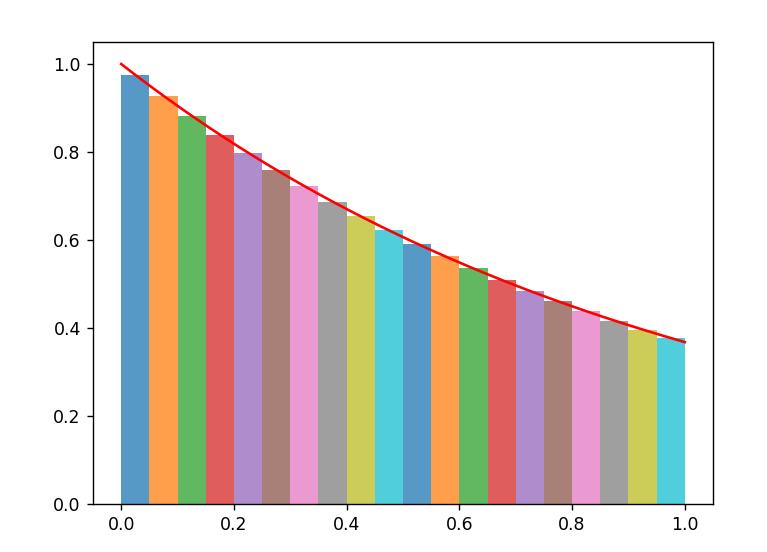
\includegraphics[width = 7.5cm, height = 4cm]{middle_200.png}\\
	\begin{tikzpicture}[remember picture,overlay]
		\node[draw,rounded corners,fill=blue!10,text width=5.5cm,align=left]
		at (10.25,4.5) {Результат:  \(R \approx 0.63211\),\\ Теор. значение: \(I \approx 0.63212\).};
	\end{tikzpicture}
	\begin{tikzpicture}[remember picture,overlay]
		\node[draw,rounded corners,fill=green!10,text width=5.5cm,align=left]
		at (10.15,2.5) {Формула погрешности:	\[|R_n| \leq max_{x \in [a, b]} |f^{\prime\prime}(x)| \frac{(b-a)^3}{24n^2}\]};
	\end{tikzpicture}
	n = 20. Ранг разбиения 0.05.
	Тогда имеем:
	\[|R_n| \leq max_{x \in [0, 1]} |e^{-x}| \frac{1}{24n^2} = \frac{1}{24n^2}\]\\
	$\bullet$При n = 20, \(|R_n| \leq 0.00010...\), \(|I - R|\approx 0.00001 \leq R_n\). Т.е. погрешность рассчетов не превышает максимальную.
	
	$\bullet$Отметим, что \(e^{-x} \in C^2[0, 1]\), так что все 4 полученные оценки погрешности корректны. Для всех четырех методов выполняется: \(|R_n| \xrightarrow{n \to \infty}{} 0\).
	\end{frame}
	
	\large \textbf{\textcolor{structure.fg}{Индивидуальная часть. Ушаков Роман}}\\
	Дан интеграл:
	\(\int\limits_0^{\pi/2} \cos{2x} \, dx\)
	
	Для нахождения суммы для интеграла Римана на \([a, b]\) воспользуемся формулой левых прямоугольников:
	\[\lim\limits_{n\to\infty}\frac{b-a}{n}\sum^{n-1}_{i=0}{f(x^i)}\]
	
	В нашем случае:
	\[I=\lim\limits_{n\to\infty}\frac{\pi/2}{n}\sum^{n-1}_{k=0}{\cos{(2k \cdot \frac{\pi/2}{n})}} = \frac{\sin(n \alpha /2)}{\sin(\alpha / 2)} \cdot \cos(\frac{(n-1)\alpha}{2}), \text{ при } \sin(\alpha/2) \neq 0.\]
	\textbf{Вычисление суммы}
	Подставляем(\(\alpha = \frac{\pi}{n}\)):
	\(I=\lim\limits_{n\to\infty} (\frac{\pi/2}{n} \cdot \frac{\sin(\pi/2)}{\sin(\frac{\pi}{2n})} \cdot \sin(\frac{\pi}{2n}))=\lim\limits_{n\to\infty}\frac{\pi/2}{n}=0\)
	
	
	\newpage

	
	
	3. \textbf{Проверка существования интеграла}
	
	Данная функция \(\cos(2x)\) непрерывна на отрезке \([a, b]\), что является достаточным условием для существования интеграла.
	
	\vspace{0.2cm}
	
	4. \textbf{Проверка прямым интегрированием}
	
	\[\int\limits_0^{\pi/2} \cos{2x} \, \left.dx=\frac{1}{2}\sin(2x)\right|_0^{\pi/2}=\frac{1}{2}\sin(\pi)-\frac{1}{2}\sin(0)=0.\]
	\large \textbf{\textcolor{structure.fg}{Часть 2. Численное интегрирование}}\\
	
	$\bullet$Язык программирования - Python.\\
$\bullet$Отрисовка графиков по посчитанным точкам - библиотека matplotlib\\
$\bullet$Значение определенного интеграла: \(I=0\)\\[1cm]
$\bullet$	\(\cos{2x} \in C^2[0, \pi/2]\), так что все следующие полученные оценки погрешности корректны. 
	
	\newpage
	
	\large \textbf{\textcolor{structure.fg}{Метод левых прямоугольников}}\\
	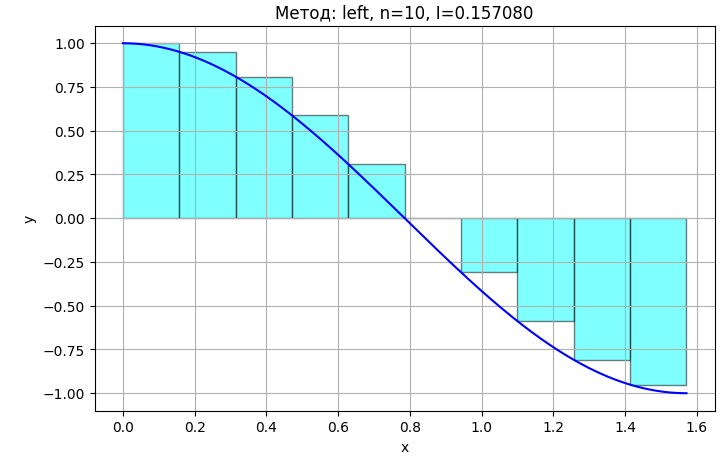
\includegraphics[width=7.5cm]{left_n10.png}\\
	\begin{tikzpicture}[remember picture,overlay]
		\node[draw,rounded corners,fill=blue!10,text width=5.5cm,align=left]
		at (10.25,4.5) {Результат: \(R = 0.157080\),\\ Теор. значение: \(I=0\).};
	\end{tikzpicture}
	\begin{tikzpicture}[remember picture,overlay]
		\node[draw,rounded corners,fill=green!10,text width=5.5cm,align=left]
		at (10.15,2.5) {Формула погрешности:\[|R_n| \leq \max_{x \in [a, b]} |f^\prime(x)| \frac{(b-a)^2}{2n}\]};
	\end{tikzpicture}
	\(n=10\) \\
	\(|R_n|\leq \max\limits_{x\in[0,\pi/2]}{|-2\sin{2x}|\frac{(\pi/2)^2}{2n}}=\frac{\pi^2}{4n}\) \\
	Погрешность: \(|R_n|\leq \frac{\pi^2}{4n}=\frac{\pi^2}{4\cdot 10} \approx 0.246740\), \(|R-I|\approx0.157080 \leq R_n\),\\
	погрешность расчетов не превышает теоретическую.
	
	\newpage
	
	\large \textbf{\textcolor{structure.fg}{Метод правых прямоугольников}}\\
	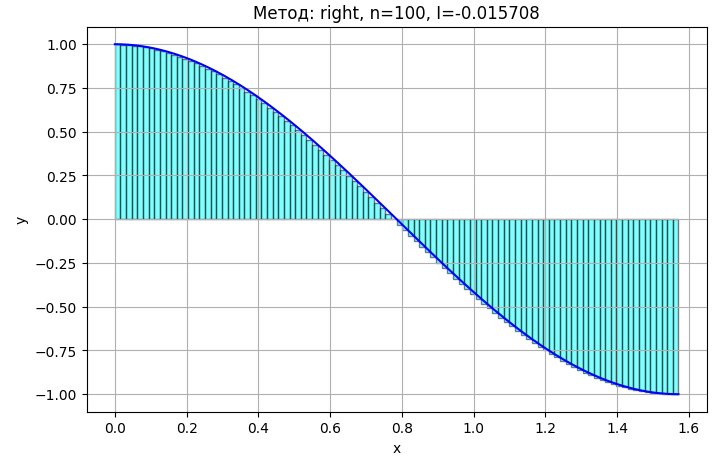
\includegraphics[width=7.5cm]{right_n100.png}\\
	\begin{tikzpicture}[remember picture,overlay]
		\node[draw,rounded corners,fill=blue!10,text width=5.5cm,align=left]
		at (10.25,4.5) {Результат: \( R=-0.015708\),\\ Теор. значение: \(I=0\).};
	\end{tikzpicture}
	\begin{tikzpicture}[remember picture,overlay]
		\node[draw,rounded corners,fill=green!10,text width=5.5cm,align=left]
		at (10.15,2.5) {Формула погрешности:\[|R_n| \leq \max_{x \in [a, b]} |f^\prime(x)| \frac{(b-a)^2}{2n}\]};
	\end{tikzpicture}
	\(n=100\) \\
	Погрешность: \(|R_n|\leq \frac{\pi^2}{4n}=\frac{\pi^2}{4\cdot 100} \approx 0.024674\), \(|R-I|\approx0.015708 \leq R_n\),\\
	погрешность расчетов не превышает теоретическую.

	\newpage
	
	\large \textbf{\textcolor{structure.fg}{Метод средних прямоугольников}}\\
	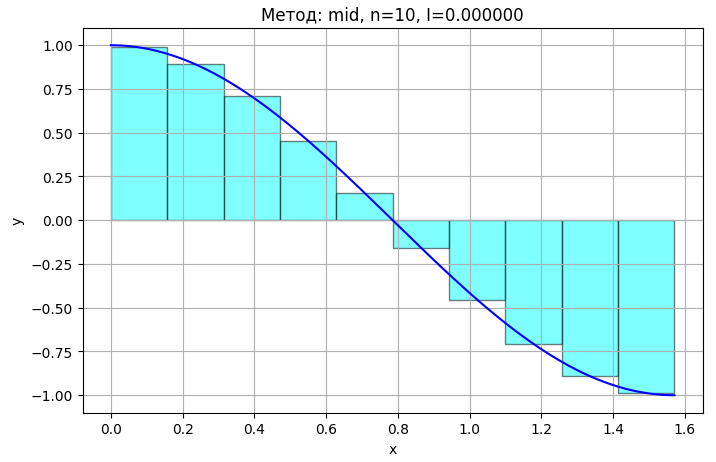
\includegraphics[width=7.5cm]{mid_n10.png}\\
	
	\begin{tikzpicture}[remember picture,overlay]
		\node[draw,rounded corners,fill=blue!10,text width=5.5cm,align=left]
		at (10.25,4.5) {Результат: \(R=0\),\\ Теор. значение: \(I=0\).};
	\end{tikzpicture}
	\begin{tikzpicture}[remember picture,overlay]
		\node[draw,rounded corners,fill=green!10,text width=5.5cm,align=left]
		at (10.15,2.5) {Формула погрешности:\[|R_n|\leq \max\limits_{x\in[a,b]}{|f''(x)|\frac{(b-a)^3}{24n^2}}\]};
	\end{tikzpicture}
	
	
	\(n=10\) \\
	\(|R_n| \leq \max\limits_{x\in[0,\pi/2]}{|-4\cos{2x}|\frac{(\pi/2)^3}{24n^2}}=\frac{\pi^3}{48n^2}\)\\
	Погрешность: \(|R_n|\leq \frac{\pi^3}{48n^2}=\frac{\pi^3}{48\cdot 100} \approx 0.006459\),  \(|R-I| \approx 0  \leq R_n\),\\
	погрешность расчетов не превышает теоретическую.
	
	\newpage
	
	\large \textbf{\textcolor{structure.fg}{Метод трапеций}}\\
	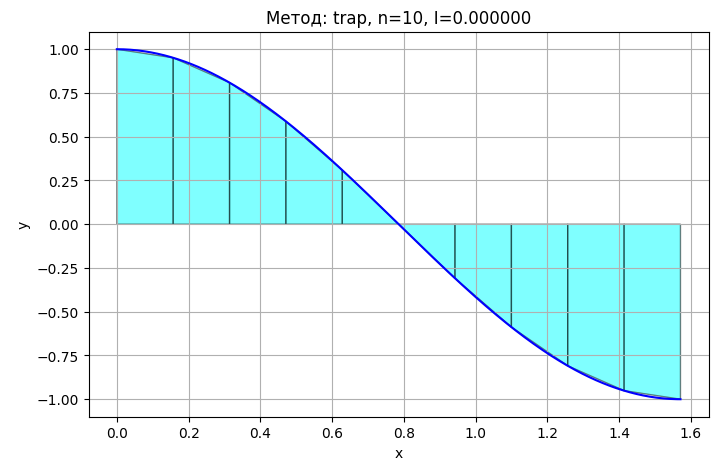
\includegraphics[width=7.5cm]{trap_n10.png}\\
	\begin{tikzpicture}[remember picture,overlay]
		\node[draw,rounded corners,fill=blue!10,text width=5.5cm,align=left]
		at (10.25,4.5) {Результат: \(R=0\),\\ Теор. значение: \(I=0\).};
	\end{tikzpicture}
	\begin{tikzpicture}[remember picture,overlay]
		\node[draw,rounded corners,fill=green!10,text width=5.5cm,align=left]
		at (10.15,2.5) {Формула погрешности:\[|R_n|\leq \max\limits_{x\in[a,b]}{|f''(x)|\frac{(b-a)^3}{12n^2}}\]};
	\end{tikzpicture}
	
	\(n=10,\) \\
	Погрешность: \(|R_n| \leq \frac{\pi^3}{24n^2}=\frac{\pi^3}{24\cdot 100} \approx 0.0129192\), \(|R-I| \approx 0 \leq R_n\),\\
	погрешность расчетов не превышает теоретическую.\\
	
	Отметим, что для всех четырех методов выполняется: \(|R_n| \xrightarrow{n \to \infty}{} 0\).
	\newpage
	\large \textbf{\textcolor{structure.fg}{Сравнительный анализ представленных методов}}\\[0.5cm]
	$\bullet$\textcolor{orange}{Методы левых и правых прямоугольников} имеют почти одинаковую погрешность(разность между ними относительно мала, так что ее можно считать за погрешность).\\
	$\bullet$\textcolor{orange}{Методы трапеций и средних прямоугольников} имеют гораздо большую точность в сравнении с первыми двумя, при том же n=10.\\[0.5cm]
	
	$\bullet$\textcolor{orange}{Метод трапеции лучше апроксимирует функцию}(чем больше n, тем больше трапеции похожи на функцию).\\
	$\bullet$\textcolor{orange}{Метод средних прямоугольников имеет наименьшую ошибку} за счет того, что погрешности на концах интервалов частично компенсируют друг друга.
	\newpage
	\large \textbf{\textcolor{structure.fg}{Индивидуальная часть. Веселов Фёдор}}\\
	
	\textbf{Дан интеграл функции: } \(\int_{0}^{\pi}  \sin{x} dx\)\\
	Формула правых прямоугольников для f(x) = $\sin{x}$, разбиение равномерное:\\
	\[\lim_{n \to \infty}\frac{b-a}{n}*\sum_{i=1}^{n}f(x_i) = \lim_{n \to \infty}\frac{\pi}{n}\sum_{k=1}^n sin(\frac{k\pi}{n})\]\\
	\textbf{Нахождение интегральной суммы} (переход (*) подробно описан в рассчетном файле)
	\[
	\lim_{n \to \infty} \frac{\pi}{n}\sum_{k=1}^n sin(\frac{k\pi}{n}) =
	\lim_{n \to \infty} \frac{\pi}{n}\sum_{k=1}^n \frac{sin(\frac{k\pi}{n})\cdot2\sin(\frac{\pi}{n})}{2\sin(\frac{\pi}{n})} 
	\overset{(*)}{=}\]\[\overset{(*)}{=}\lim_{n \to \infty} \frac{\pi}{n}\Biggl( 
	\frac{\cos\Bigl(\frac{\pi}{2n}\Bigr) - \cos\Bigl(\pi+\frac{\pi}{2n}\Bigr)}{2\sin(\frac{\pi}{2n})} \Biggr) = \lim_{n \to \infty} \underbrace{\frac{\frac{\pi}{2n}}{\sin(\frac{\pi}{2n})}}_{\to1} \cdot 
	\underbrace{2\cos\left(\frac{\pi}{2n}\right)}_{\to 2} = \boxed{2}
	\]
	\newpage
	\textbf{Доказательство существования интеграла}\\
	Функция f(x) = sin(x) непрерывна на отрезке  $[0,\pi]$ , а следовательно по критерию интегрируемости Римана она интегрируема.
	
	\textbf{Нахождение через определенный интеграл}
	\[
	\int_0^\pi f(x) \, dx = \int_0^\pi sin(x) \, dx = \Bigl[-cos(x)\Bigr]\Bigg|_0^\pi = 2 
	\]
	Значения интеграла вычисленные разными способами совпадают.\\
	\large \textbf{\textcolor{structure.fg}{Графики интегральных сумм}}\\
		$\bullet$Язык программирования - Python.\\
	$\bullet$Отрисовка графиков по посчитанным точкам - библиотека matplotlib\\
	$\bullet$Значение определенного интеграла: \(I=2\)\\[1cm]
	$\bullet$	\(sin{x} \in C^2[0, \pi]\), так что все следующие полученные оценки погрешности корректны. 
	\newpage
	
	\textbf{Метод левых прямоугольников}\\
	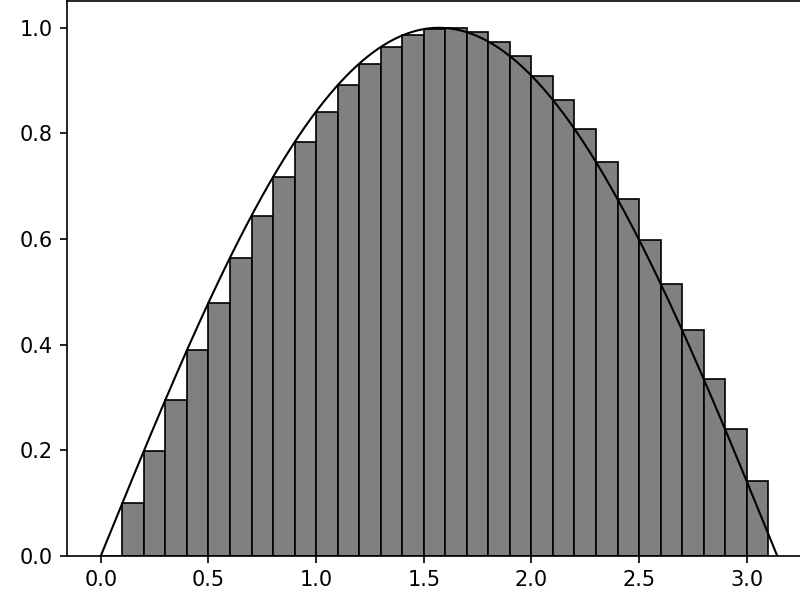
\includegraphics[width=7.5cm]{Sin_left.png}
	
	\begin{tikzpicture}[remember picture,overlay]
		\node[draw,rounded corners,fill=blue!10,text width=5.5cm,align=left]
		at (10.25,4.5) {Результат: \(R = 1.9953899\),\\ Теор. значение: \(I=2\).};
	\end{tikzpicture}
	\begin{tikzpicture}[remember picture,overlay]
		\node[draw,rounded corners,fill=green!10,text width=5.5cm,align=left]
		at (10.15,2.5) {Формула погрешности:\[|R_n| \le \max_{x \in [a, b]} |f'(x)| \frac{(b - a)^2}{2n}\]};
	\end{tikzpicture}
	n = 31; Ранг разбиения: 0.1.\\
	В нашем случае: 
	$|R_n| \le \max_{x \in [0, \pi]} |-sin(x)| \frac{\pi^2}{2n} = \frac{\pi^2}{2n} $
	$ n = 31 \implies R_n \leq \frac{\pi^2}{62} < 0.15919$
	$ |I - R| \approx 0,0046101 < R_n \implies \text{Рассчитано корректно}$
	\newpage
	
	
	\textbf{Метод правых прямоугольников}
	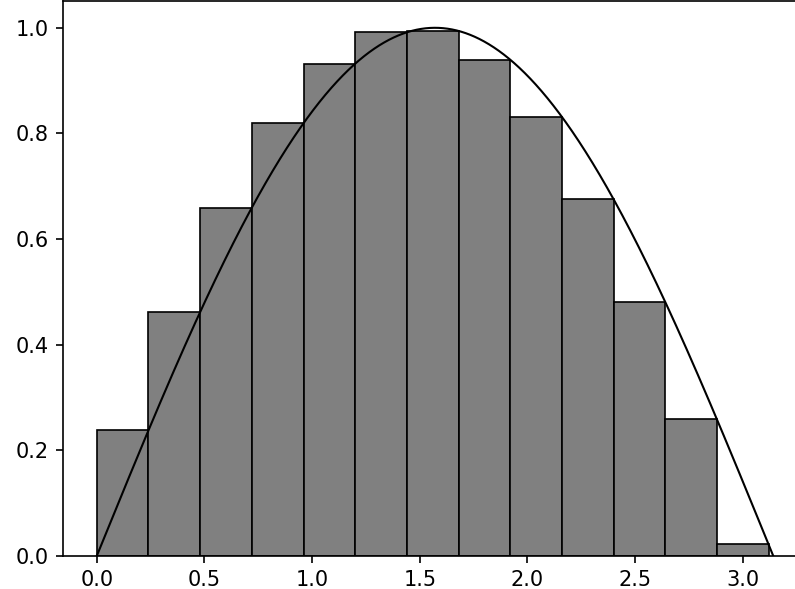
\includegraphics[width=7.5cm]{Sin_right.png}
	
	\begin{tikzpicture}[remember picture,overlay]
		\node[draw,rounded corners,fill=blue!10,text width=5.5cm,align=left]
		at (10.25,4.5) {Результат: \(R \approx 1.992749\),\\ Теор. значение: \(I=2\).};
	\end{tikzpicture}
	\begin{tikzpicture}[remember picture,overlay]
		\node[draw,rounded corners,fill=green!10,text width=5.5cm,align=left]
		at (10.15,2.5) {Формула погрешности:\[|R_n| \le \max_{x \in [a, b]} |f'(x)| \frac{(b - a)^2}{2n}\]};
	\end{tikzpicture}
	\\n = 13; Ранг разбиения: 0.24.
	В нашем случае: 
	$|R_n| \le \max_{x \in [0, \pi]} |cos(x)| \frac{\pi^2}{2n} = \frac{\pi^2}{2n} $
	$ n = 13 \implies R_n \leq \frac{\pi^2}{26} < 0.37960017$ 
	$ |I - R| = 0.007250304 < R_n \implies \text{Рассчитано корректно}$
	\newpage
	\textbf{Метод средних прямоугольников}
	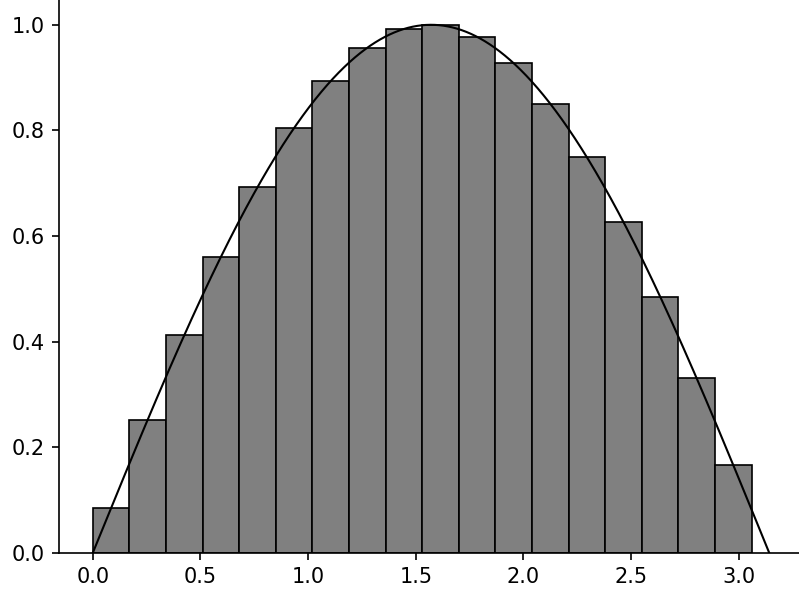
\includegraphics[width=7.5cm]{Sin_middle.png}
	
	\begin{tikzpicture}[remember picture,overlay]
		\node[draw,rounded corners,fill=blue!10,text width=5.5cm,align=left]
		at (10.25,4.5) {Результат: \(R \approx 1.999079\),\\ Теор. значение: \(I=2\).};
	\end{tikzpicture}
	\begin{tikzpicture}[remember picture,overlay]
		\node[draw,rounded corners,fill=green!10,text width=5.5cm,align=left]
		at (10.15,2.5) {Формула погрешности:\[|R_n| \le \max_{x \in [a, b]} |f''(x)| \frac{(b - a)^3}{24n^2}\]};
	\end{tikzpicture}
	
	В нашем случае: 
	$|R_n| \le \max_{x \in [0, \pi]} |cos(x)| \frac{\pi^3}{24n^2} = \frac{\pi^3}{24n^2} $
	$ n = 18 \implies R_n \leq \frac{\pi^3}{7776} < 0,003987 $
	$ |I - R| \approx 0.00092 < R_n \implies \text{Рассчитано корректно}$
	\newpage
	\textbf{Метод трапеций}\\
	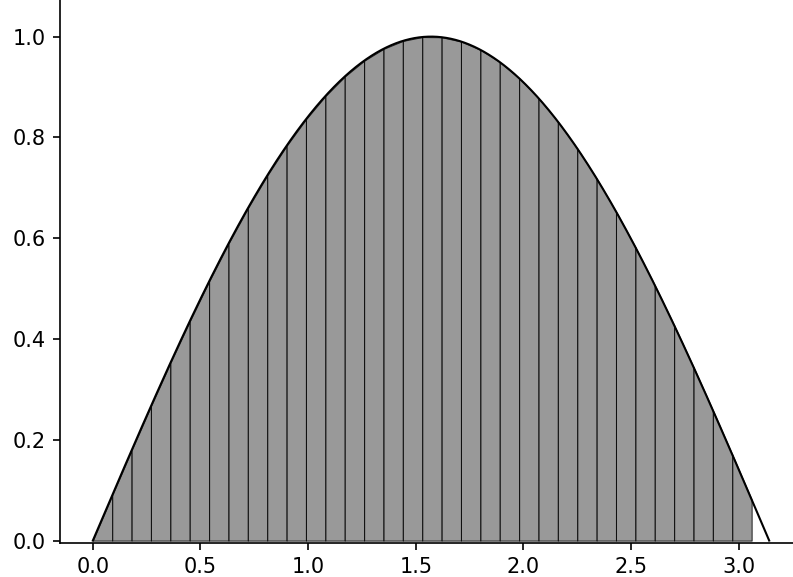
\includegraphics[width=7.5cm]{Sin_trap.png}
	
	\begin{tikzpicture}[remember picture,overlay]
		\node[draw,rounded corners,fill=blue!10,text width=5.5cm,align=left]
		at (10.25,4.5) {Результат: \(R \approx 1.995325\),\\ Теор. значение: \(I=2\).};
	\end{tikzpicture}
	\begin{tikzpicture}[remember picture,overlay]
		\node[draw,rounded corners,fill=green!10,text width=5.5cm,align=left]
		at (10.15,2.5) {Формула погрешности:\[|R_n| \le \max_{x \in [a, b]} |f''(x)| \frac{(b - a)^3}{12n^2}\]};
	\end{tikzpicture}
	n = 34; Ранг разбиения: 0.09.\\
	В нашем случае: 
	$|R_n| \le \max_{x \in [0, \pi]} |-cos(x)| \frac{(\pi - 0)^3}{12n^2} = \frac{\pi^3}{12n^2} $
	$ n = 34 \implies R_n \leq \frac{\pi^3}{13872} < 0,0032351 $
	$ |S_\text{ист} - S_\text{гр}| = 0.003174771 < R_n \implies \text{Рассчитано корректно}$
	\newpage
	\textcolor{structure.fg}{\textbf{Сравнительный анализ}}\\
	
	\begin{tabular}{|c|c|c|c|}
		\hline
		\textbf{\makecell{Название\\метода}} & \textbf{S} & \textbf{Погрешность}& \textbf{\makecell{Относительная\\погрешность}} \\
		\hline
		 \makecell{Левых\\ прямоугольников} & 1,995389893 & 0,0046101066 & 0,231\% \\
		\hline
		 \makecell{Правых\\прямоугольников} & 1,999547959 & 0,0004520403 & 0,022\% \\
		\hline
		 \makecell{Средних\\прямоугольников} & 1,999968366 & 0,0000316338 & 0,002\% \\
		\hline
		 \makecell{Левых\\прямоугольников}& 1,997468926 & 0,0025310735 & 0,126\% \\
		\hline
	\end{tabular}
	
	При ранге разбиения = 0.1:\\
	$\bullet$ \textcolor{orange}{самый точный метод} - средние прямоугольники\\ (отн.погрешность < 0,01\%)\\
	$\bullet$ \textcolor{orange}{Cамый неточный} - левые прямоугольники\\ (отн.погрешность > 0,2\%)
	
	\newpage
	\large \textbf{\textcolor{structure.fg}{Индивидуальная часть. Босенко Борис}}\\
	
		Дан интеграл:
	\(\int\limits_1^{2} x^2 \, dx\)
	
	Тогда предел интегральных сумм Римана будет выглядеть как 
	\[I = \lim_{\Delta x \to 0} \sum_{k=1}^{n} f(\xi_k)\Delta x \]
	
	Так как разбиение равномерное, для числа разбиений n можем посчитать координаты точек разбиения по формуле
	
	\(x_k = 1 + \frac{k}{n} ( 2 - 1 ) = 1 + \frac{k}{n}, k \in \{0, ..., n\}\)

	Тогда можем посчитать данный интеграл с помощью \textcolor{orange}{формулы правых прямоугольников:}
	
	\[ I = \lim_{\frac{1}{n} \to 0} \sum_{k=1}^{n} \left( f\left(1 + \frac{k}{n}\right) \frac{1}{n} \right) =1 + \lim_{n \to \infty} \frac{n+1}{n} + \lim_{n \to \infty} \frac{2n^2 + 3n + 1}{6n^2} = \frac{7}{3}\]
	\newpage
	\textbf{Доказательство существования интеграла}\\
Функция $f(x) = x^2$ интегрируема на промежутке $[1, 2]$, так как она непрерывна, а следовательно по критерию интегрируемости Римана она интегрируема.
	
	\textbf{Нахождение через определенный интеграл}
	
	\[ \int_{1}^{2} f(x) dx = \int_{1}^{2} x^2 dx = \frac{x^3}{3} \ \bigg|_{1}^{2} = \frac{7}{3}\]
	
	Таким образом, \textcolor{orange}{оба способа дали одинаковый результат}.
	
	\large \textbf{\textcolor{structure.fg}{Графики интегральных сумм}}\\
	$\bullet$Язык программирования - Python.\\
	$\bullet$Отрисовка графиков по посчитанным точкам - библиотека matplotlib\\
	$\bullet$Значение определенного интеграла: \(I=\frac{7}{3}\approx 2.3333\)\\[1cm]
	$\bullet$	\(x^2 \in C^2[1, 2]\), так что все следующие полученные оценки погрешности корректны.
	
	\addcontentsline{toc}{chapter}{Результаты работы программы}
	\large \textbf{\textcolor{structure.fg}{Метод правых прямоугольников}}
	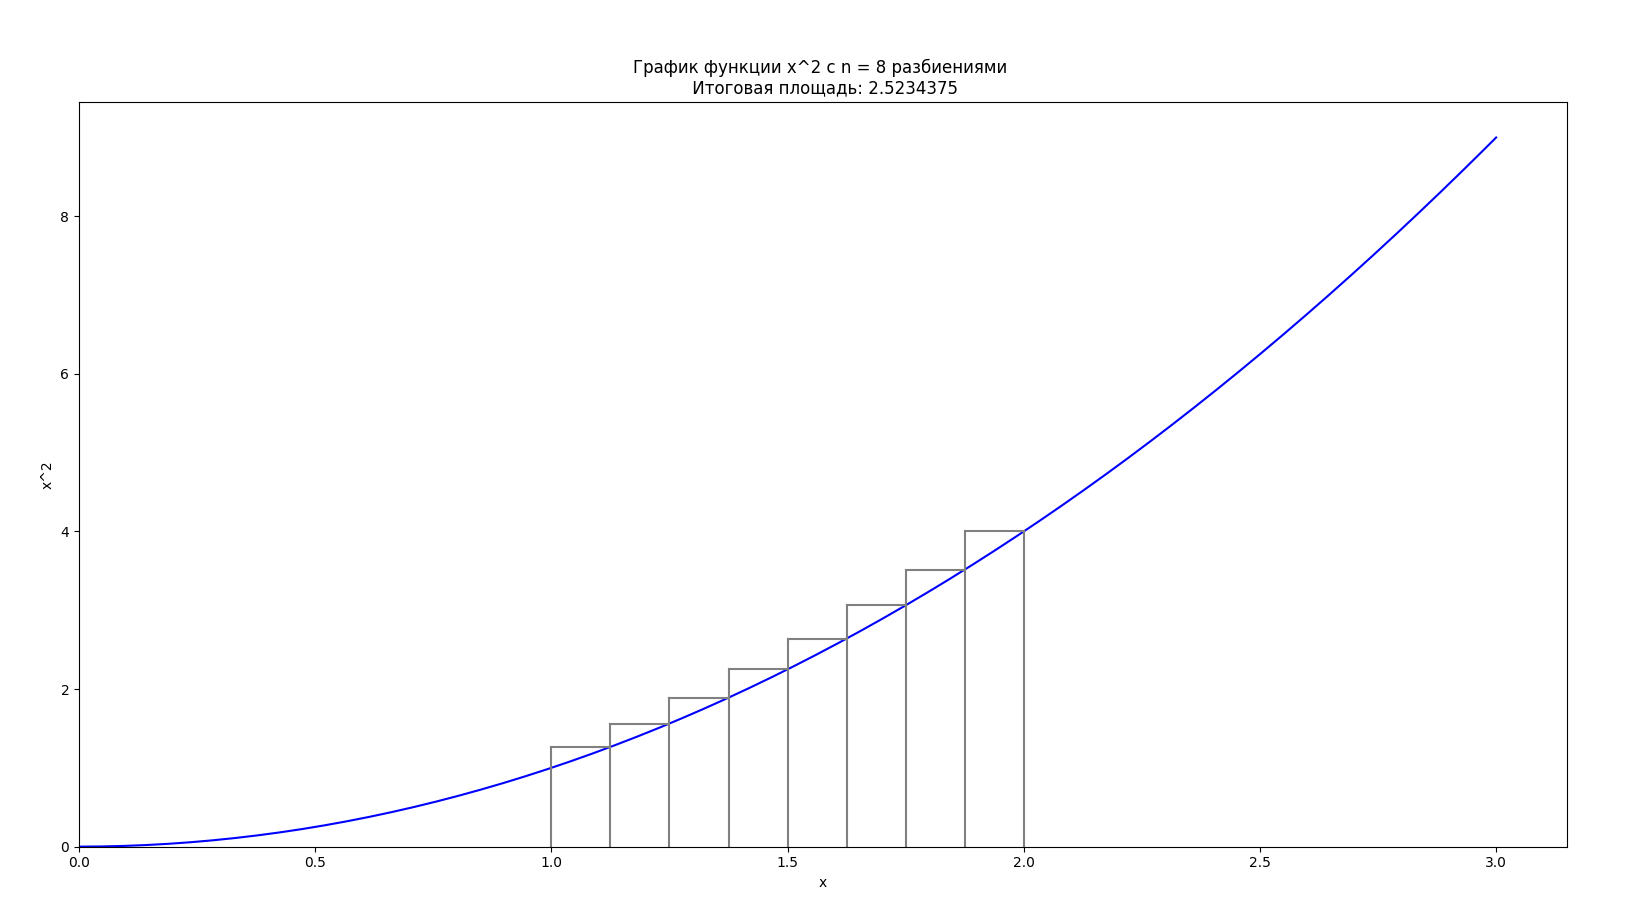
\includegraphics[width=7.5cm]{Правые прямоугольники.png}\\
	\begin{tikzpicture}[remember picture,overlay]
		\node[draw,rounded corners,fill=blue!10,text width=5.5cm,align=left]
		at (10.25,4.5) {Результат: \(R \approx 2.5234375\),\\ Теор. значение: \(I=2.3333\).};
	\end{tikzpicture}
	\begin{tikzpicture}[remember picture,overlay]
		\node[draw,rounded corners,fill=green!10,text width=5.5cm,align=left]
		at (10.15,2.5) {Формула погрешности:\[|R_n| \le \max_{x \in [a, b]} |f'(x)| \frac{(b - a)^2}{2n}\]};
	\end{tikzpicture}
	$\bullet$Для правых прямоугольников при n = 8 по формуле погрешность не превышает
	
	\[ 4 \cdot \frac{(2 - 1)^2}{2 \cdot 8} = \frac{1}{4}\]
	
	На графике погрешность равна $\left| \frac{8 - 1}{3} - 2.5234375 \right| \approx 0.1901042$, что \textcolor{orange}{соответствует теоретической погрешности}.
	\newpage
	\large \textbf{\textcolor{structure.fg}{Метод левых прямоугольников}}
		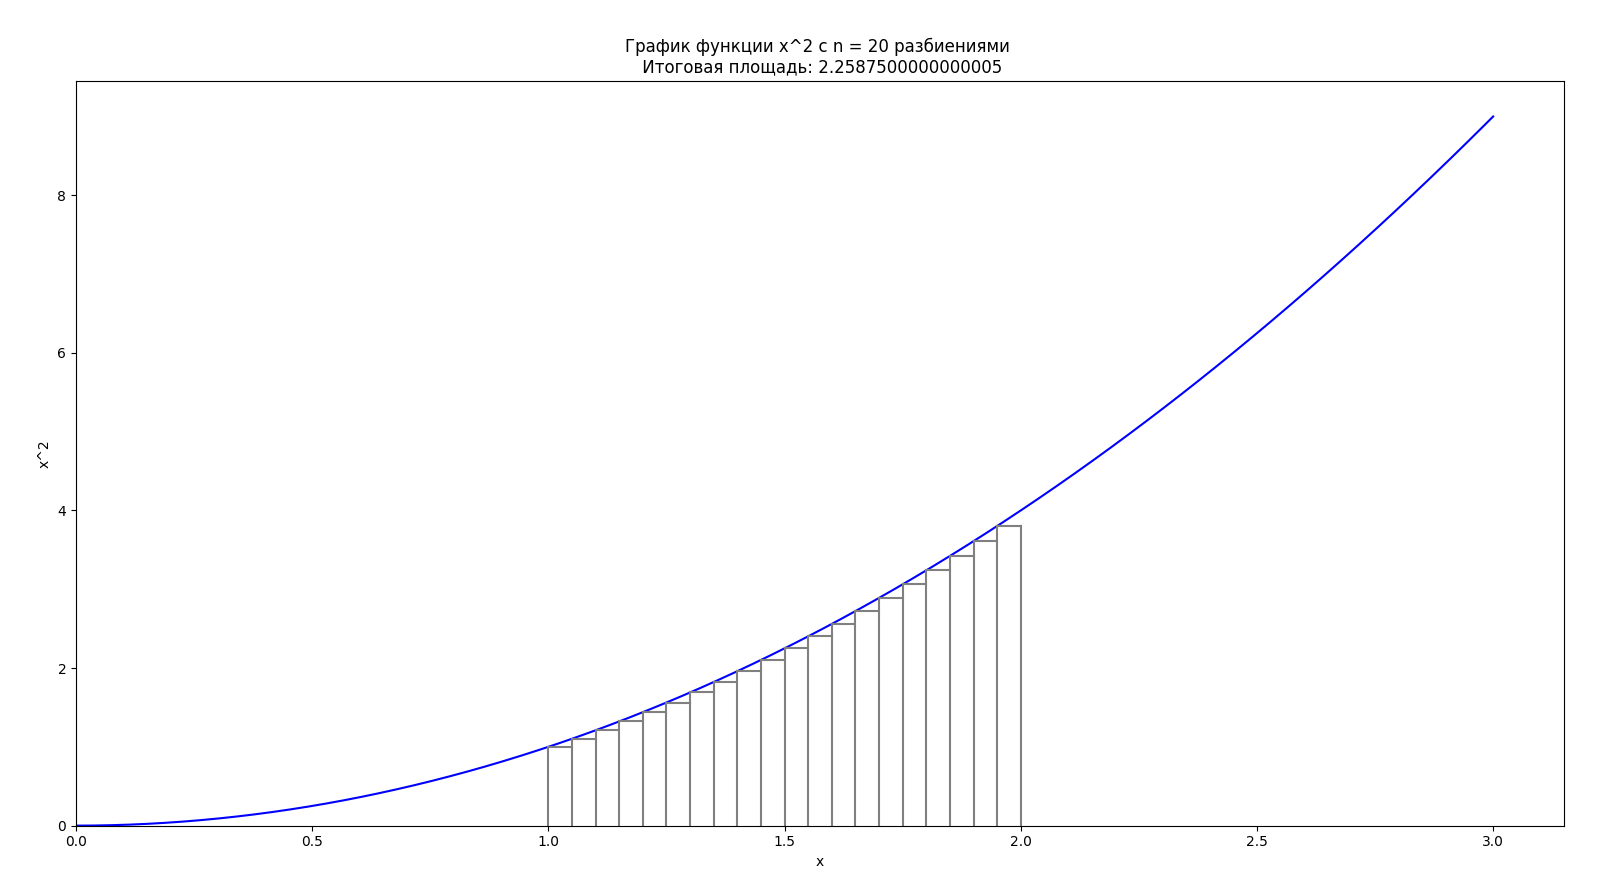
\includegraphics[width=7.5cm]{Левые прямоугольники.png}\\
	\begin{tikzpicture}[remember picture,overlay]
		\node[draw,rounded corners,fill=blue!10,text width=5.5cm,align=left]
		at (10.25,4.5) {Результат: \(R \approx 2.25875\),\\ Теор. значение: \(I=2.3333\).};
	\end{tikzpicture}
	\begin{tikzpicture}[remember picture,overlay]
		\node[draw,rounded corners,fill=green!10,text width=5.5cm,align=left]
		at (10.15,2.5) {Формула погрешности:\[|R_n| \le \max_{x \in [a, b]} |f'(x)| \frac{(b - a)^2}{2n}\]};
	\end{tikzpicture}
	$\bullet$Для правых прямоугольников при n = 8 по формуле погрешность не превышает
	
	\[ 4 \cdot \frac{(2 - 1)^2}{2 \cdot 8} = \frac{1}{4}\]
	
	На графике погрешность равна $\left| \frac{8 - 1}{3} - 2.25875 \right| \approx 0.07458$, что \textcolor{orange}{соответствует теоретической погрешности}.
	\newpage
	\large \textbf{\textcolor{structure.fg}{Метод трапеций}}\\
	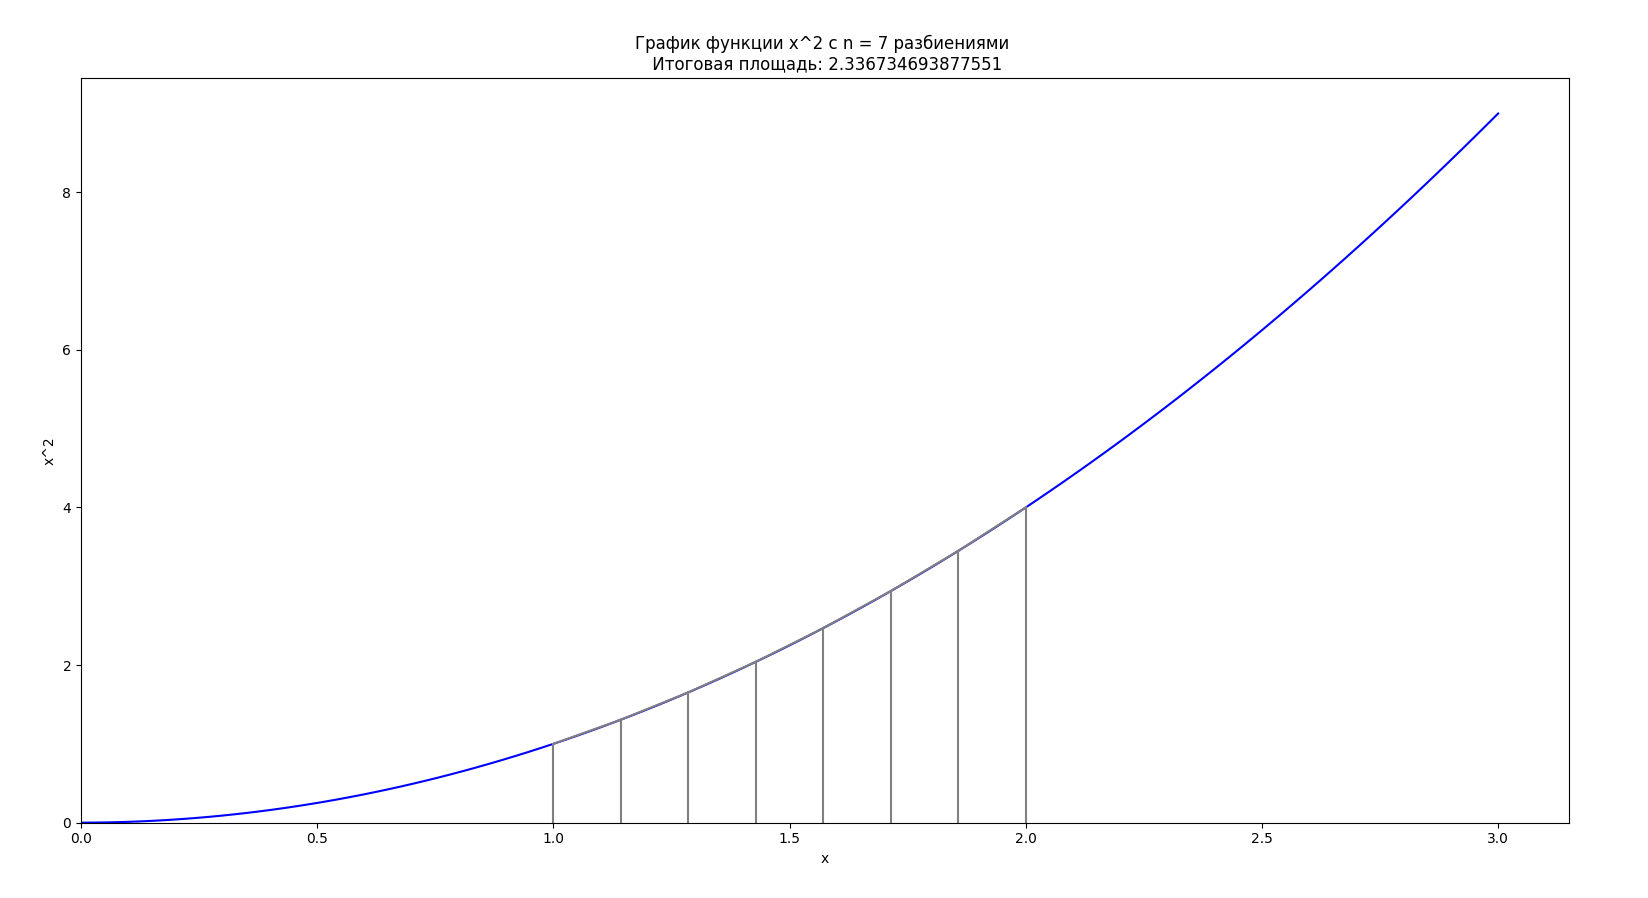
\includegraphics[width=7.5cm]{Трапеции.png}\\
	\begin{tikzpicture}[remember picture,overlay]
		\node[draw,rounded corners,fill=blue!10,text width=5.5cm,align=left]
		at (10.25,4.5) {Результат: \(R \approx 2.33673469\),\\ Теор. значение: \(I=2.3333\).};
	\end{tikzpicture}
	\begin{tikzpicture}[remember picture,overlay]
		\node[draw,rounded corners,fill=green!10,text width=5.5cm,align=left]
		at (10.15,2.5) {Формула погрешности:\[|R_n| \le \max_{x \in [a, b]} |f''(x)| \frac{(b - a)^3}{12n^2}\]};
	\end{tikzpicture}
$\bullet$Для трапеций при n = 7 по формуле погрешность не превышает

\[ 2 \cdot \frac{(2 - 1)^3}{12 \cdot 49} = \frac{1}{147} \approx 0.0068027\]

На графике погрешность равна $\left| \frac{8 - 1}{3} - 2.33673469 \right| \approx 0.00340136$, что \textcolor{orange}{соответствует теоретической погрешности}.
	\newpage
	\large \textbf{\textcolor{structure.fg}{Метод средних прямоугольников}}
	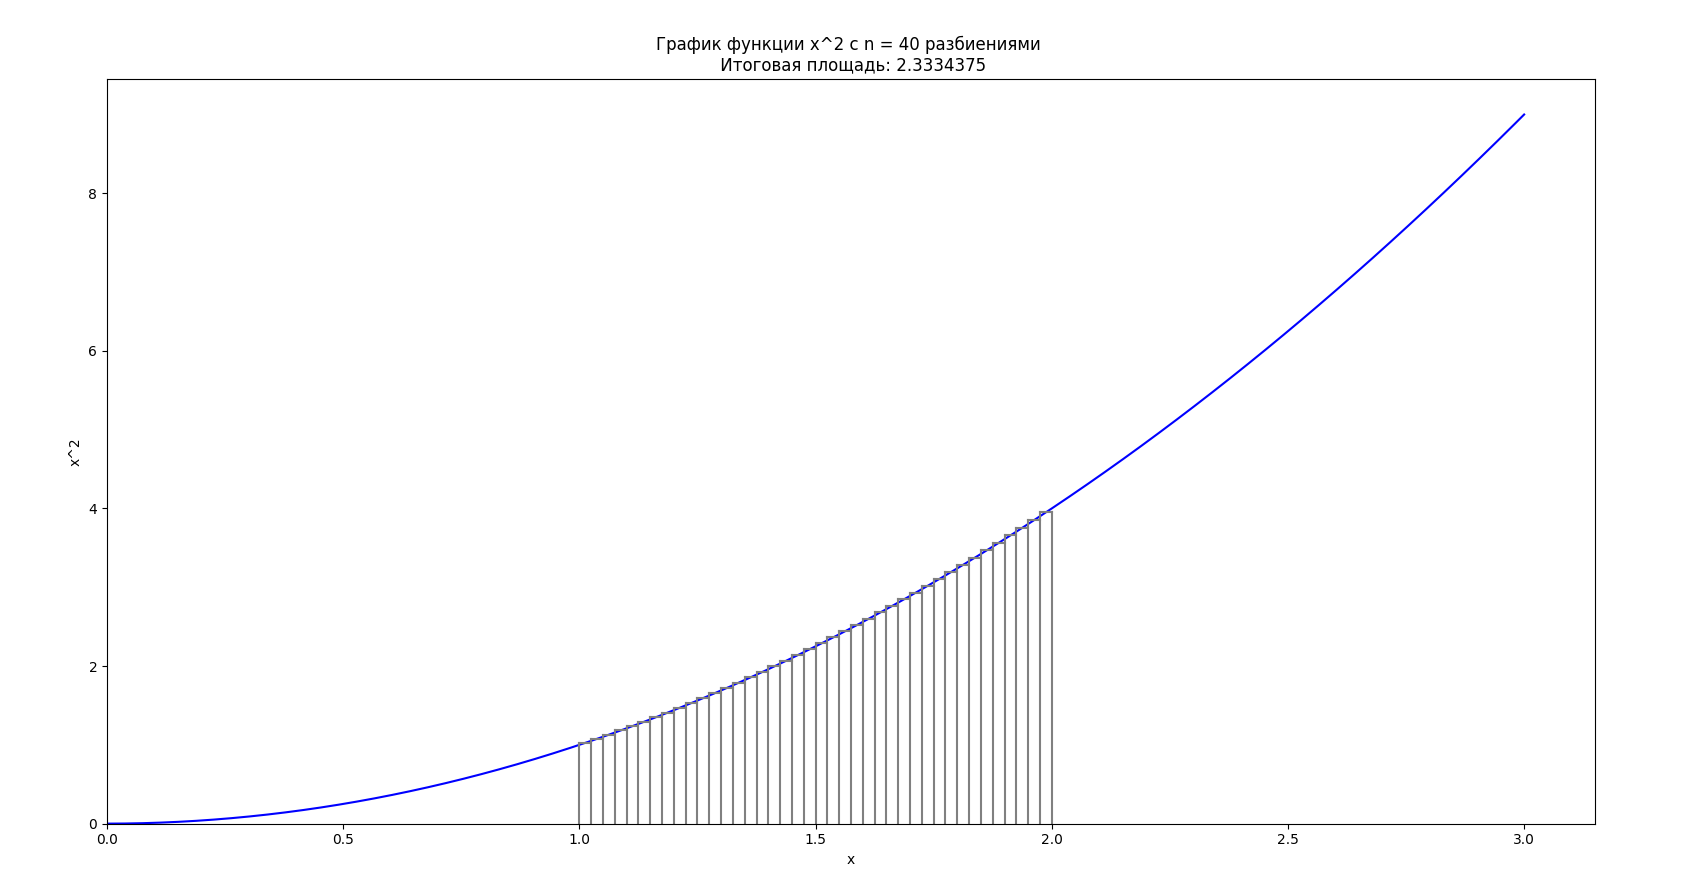
\includegraphics[width=7.5cm]{Средние прямоугольники.png}\\
	\begin{tikzpicture}[remember picture,overlay]
		\node[draw,rounded corners,fill=blue!10,text width=5.5cm,align=left]
		at (10.25,4.25) {Результат: \(R \approx 2.33673469\),\\ Теор. значение: \(I=2.3333\).};
	\end{tikzpicture}
	\begin{tikzpicture}[remember picture,overlay]
		\node[draw,rounded corners,fill=green!10,text width=5.5cm,align=left]
		at (10.15,2.25) {Формула погрешности:\[|R_n| \le \max_{x \in [a, b]} |f''(x)| \frac{(b - a)^3}{24n^2}\]};
	\end{tikzpicture}
	$\bullet$Для трапеций при n = 7 по формуле погрешность не превышает
	
	\[ 2 \cdot \frac{(2 - 1)^3}{12 \cdot 49} = \frac{1}{147} \approx 0.0068027\]
	
	На графике погрешность равна $\left| \frac{8 - 1}{3} - 2.33673469 \right| \approx 0.00340136$, что \textcolor{orange}{соответствует теоретической погрешности}.
	\newpage

	\large \textbf{\textcolor{structure.fg}{Командная часть (Малые колебания)}}\\
	\textbf{Рассчеты величин}\\
	Параметры установки: диаметр шара D = 12мм, масса M = 8г; L = 0,25м
	\[\omega = \sqrt{\frac{g}{L}}; \theta = \theta_{0} \cdot \cos(\omega t)\]
	$$g = 9,8 \frac{\text{м}}{\text{с}^2};\omega \approx 6,02464 \text{ рад/с}$$\\
	\[\text{T} = \frac{2\pi}{\omega} = 2\pi\sqrt{\frac{L}{g}} \approx 1.00354496158 c\]
	\newline
	\subsection{Таблица эксперементальных значений}
	\begin{tabular}{|l|l|l|l|} 
		\hline
		\textbf{Угол} & \textbf{Угол в радианах} & \textbf{Период} & $\Delta$\textbf{T} \\ \hline
		2.5$^\circ$ & 0.04363323 & 1.00 & 0.00354496158  \\ \hline
		5$^\circ$   & 0.08726646 & 1.02 & 0.01645503842  \\ \hline
		10$^\circ$  & 0.17453293 & 1.00 & 0.00354496158  \\ \hline
		15$^\circ$  & 0.26179939 & 1.15 & 0.14645503842 \\ \hline
	\end{tabular}
	
	\vspace{0.5cm}
	\newpage
	\textbf{Эксперименты}

	\begin{tikzpicture}[remember picture,overlay]
		
		\node[anchor=north west] at ([xshift=1cm,yshift=-0.5cm]current page.north west) {
			\begin{tabular}{c}
				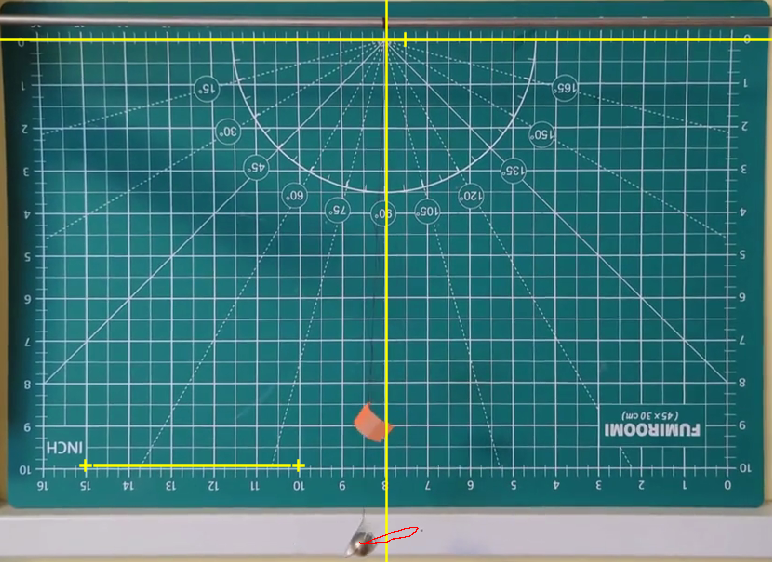
\includegraphics[width=4.5cm]{trajectory2.5.png}\\
				{\small Амплитуда 2.5$^\circ$}
			\end{tabular}
		};
		
		\node[anchor=north west] at ([xshift=7cm,yshift=-0.5cm]current page.north west) {
			\begin{tabular}{c}
				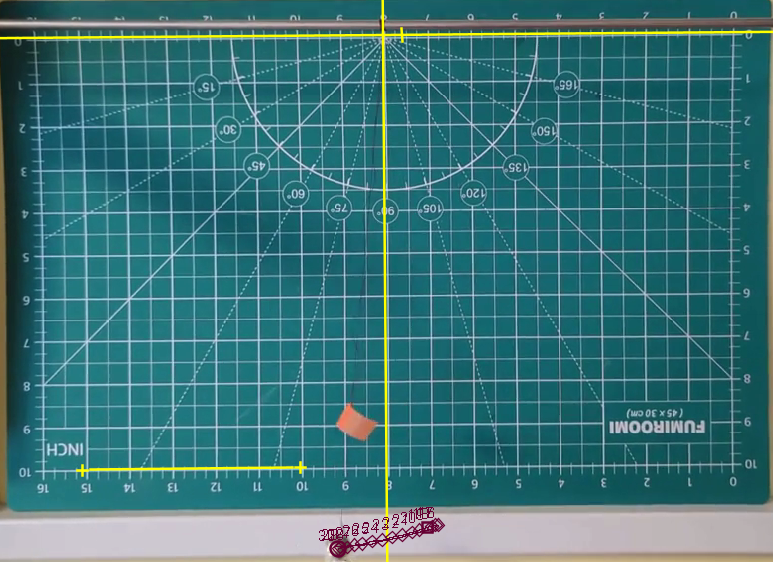
\includegraphics[width=4.5cm]{trajectory5.png}\\
				{\small Амплитуда 5$^\circ$}
			\end{tabular}
		};
		
		\node[anchor=north west] at ([xshift=1cm,yshift=-4.5cm]current page.north west) {
			\begin{tabular}{c}
				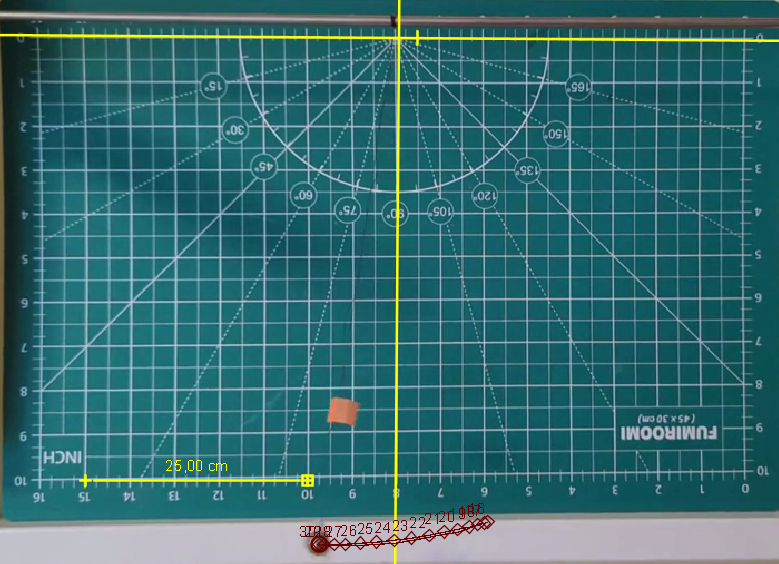
\includegraphics[width=4.5cm]{trajectory10.png}\\
				{\small Амплитуда 10$^\circ$}
			\end{tabular}
		};

		\node[anchor=north west] at ([xshift=7cm,yshift=-4.5cm]current page.north west) {
			\begin{tabular}{c}
				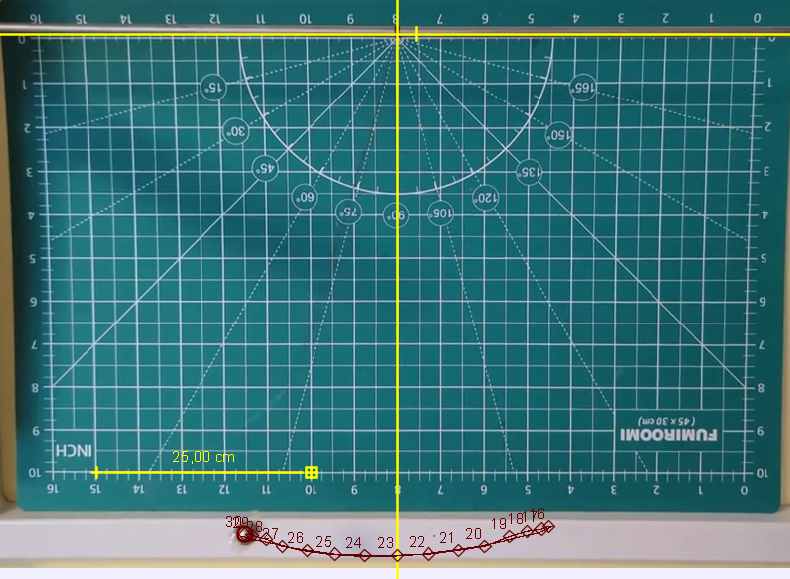
\includegraphics[width=4.5cm]{trajectory15.png}\\
				{\small Амплитуда 15$^\circ$}
			\end{tabular}
		};
		
	\end{tikzpicture}
	
	
	\newpage
	\begin{tikzpicture}[remember picture,overlay]
	\node[anchor=north west] at ([xshift=0cm,yshift=0cm]current page.north west) {
		\begin{tabular}{c}
			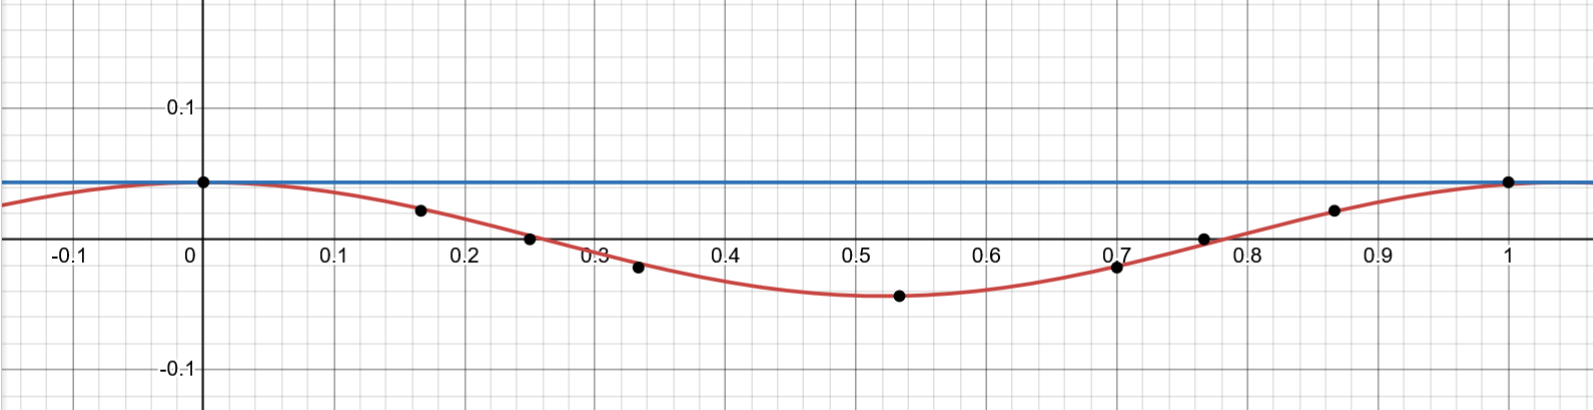
\includegraphics[width=5cm, height = 3.5cm]{Практ_2,5.png}\\
			{\small Амплитуда 2.5$^\circ$}
		\end{tabular}
	};
	
	\node[anchor=north west] at ([xshift=6cm,yshift=0cm]current page.north west) {
		\begin{tabular}{c}
			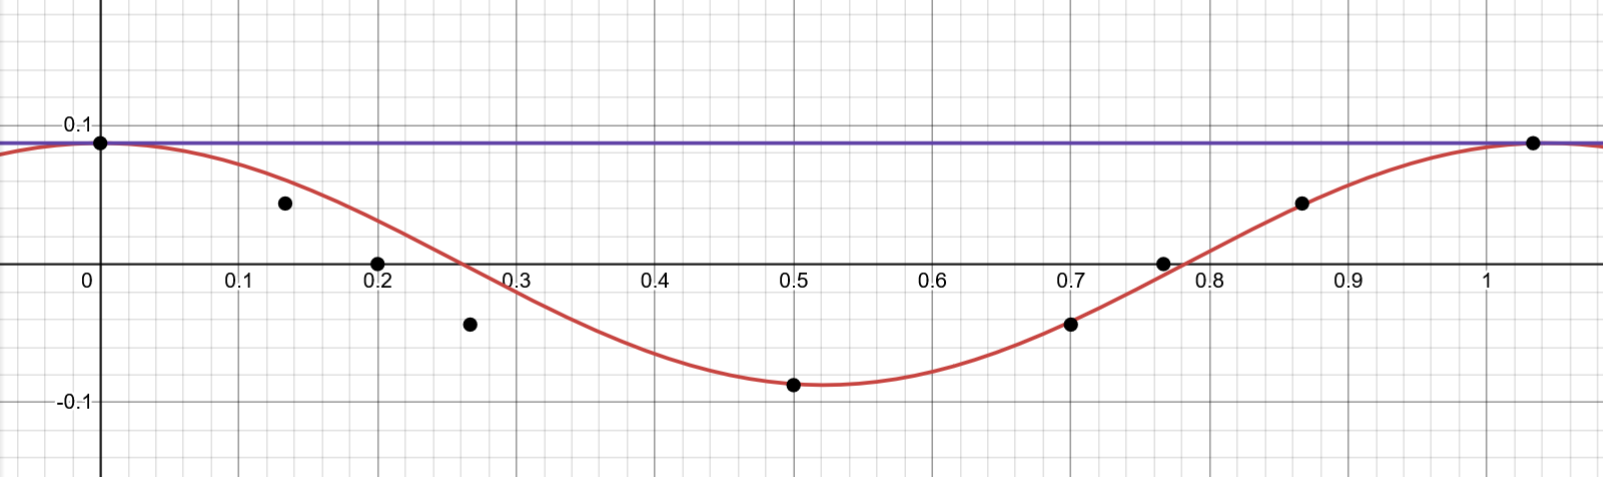
\includegraphics[width=5cm, height = 3.5cm]{Практ_5.png}\\
			{\small Амплитуда 5$^\circ$}
		\end{tabular}
	};
	
	\node[anchor=north west] at ([xshift=0cm,yshift=-4.5cm]current page.north west) {
		\begin{tabular}{c}
			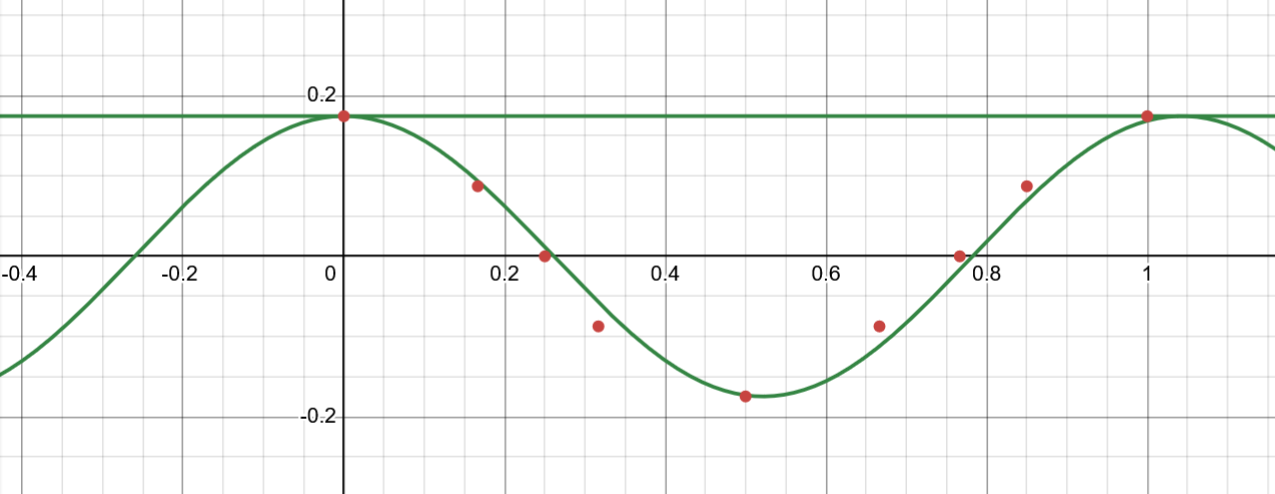
\includegraphics[width=5cm, height = 3.5cm]{Практ_10.png}\\
			{\small Амплитуда 10$^\circ$}
		\end{tabular}
	};
	
	\node[anchor=north west] at ([xshift=6cm,yshift=-4.5cm]current page.north west) {
		\begin{tabular}{c}
			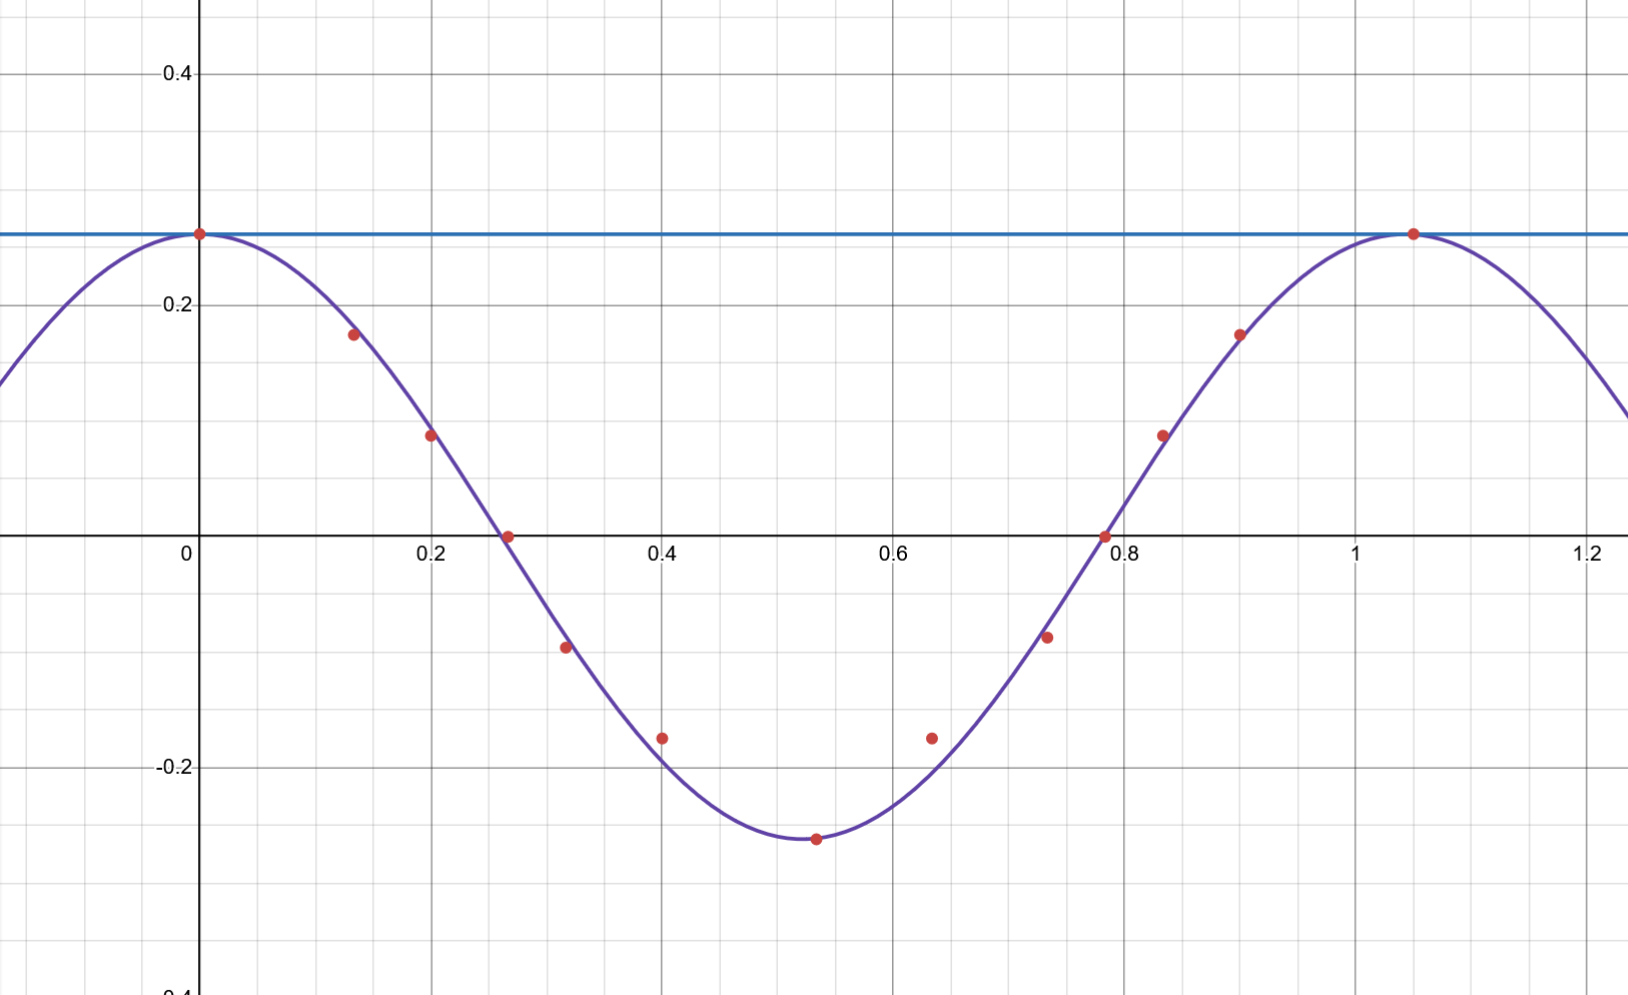
\includegraphics[width=5cm, height = 3.5cm]{Практ_15.png}\\
			{\small Амплитуда 15$^\circ$}
		\end{tabular}
	};
	
	\end{tikzpicture}
	
	\begin{tikzpicture}[remember picture,overlay]
		\node[draw,rounded corners,fill=green!10,text width=4.2cm,align=left]
		at (13,-4) {Графики зависимости от времени\\
			Точки - эксперимент,\\
		    Сплошные - теория};
	\end{tikzpicture}
	\newpage
	
	\vspace{0.5cm}
	$\bullet$ Из графиков видно что \textcolor{orange}{точность в эксперименте достаточно высока}.\\
	$\bullet$ "линейность" зависимости лучше всего проявляется в окрестности 0, что видно из графиков: при углах от 2,5 до 15 \textcolor{orange}{погрешность минимальна}.\\
	$\bullet$ Видно, что при угле 15$^\circ$ погрешность меньше чем при 5$^\circ$. Это объясняется неидеальными условиями проведения эксперимента
	
	\large \textbf{\textcolor{structure.fg}{Погрешности}}\\
	\textbf{Причины погрешности в пунктах }эксперимента:
	\begin{itemize}
	\item \textcolor{orange}{Приближение малых углов}:расчеты произведены исходя из $\sin \theta \approx \theta$. При увеличении угла (особенно к 20°) эта ошибка растет.
	\item \textcolor{orange}{Инструментальная погрешность}: Ошибка при определении момента начала и конца колебания по видео или секундомеру.
	\item \textcolor{orange}{Физические факторы}: Сопротивление воздуха и другие неучтённые воздействия.
	\end{itemize}
	\newpage
	\textbf{Рассчет погрешностей}
	\[
	\boxed{\varepsilon = \frac{|T_{\text{практ}} - T_{\text{теор}}|}{T_{\text{теор}}} \cdot 100\% = \frac{\Delta T}{T}\cdot 100\%} \]
	\begin{itemize}
	\item\(
	\varepsilon_1 = \frac{0.00354496158}{1.00354496158} \cdot 100\% \approx 0.35\% 
	\)
	\item\(
	\varepsilon_2 = \frac{0.01645503842}{1.00354496158} \cdot 100\% \approx 1.64\% 
	\)
	\item\(
	\varepsilon_3 = \frac{0.00354496158}{1.00354496158} \cdot 100\% \approx 0.35\% 
	\)
	\item\(
	\varepsilon_3 = \frac{0,14645503842}{1,00354496158} \cdot 100\% \approx 14.59\% 
	\)
\end{itemize}
	\newpage
	\textbf{Вывод}
	\begin{itemize}
	\item Экспериментально подтверждено, что для малых углов ($2{,}5^\circ$–$10^\circ$) \textcolor{orange}{линейная модель маятника описывает движение с высокой точностью} (относительная погрешность $\varepsilon < 2\%$). Это доказывает справедливость допущения $\sin \theta \approx \theta$ в данном диапазоне.
	\item Зависимость периода от амплитуды: В ходе опыта выявлено, что \textcolor{orange}{при увеличении угла до $15^\circ$ погрешность существенно возрастает} (до $14{,}59\%$), а практический период становится заметно больше теоретического. Это подтверждает, что при выходе за границы «малых углов» линейная формула начинает давать существенную ошибку.
	\item Анализ расхождений на графиках: Визуальный анализ графиков показывает, что экспериментальные точки в начале колебания практически идеально ложатся на теоретическую кривую, но \textcolor{orange}{со временем наблюдается фазовый сдвиг}. Это свидетельствует о накоплении погрешности из-за разницы периодов модели и реальности.
	\end{itemize}
	\newpage
	\large \textbf{\textcolor{structure.fg}{Командная часть (Большие колебания)}}\\
	
	\textbf{Опыты}
	
	Маятник:\\
	g - ускорение свободного падения (\(g=9.81\text{ м/c}^2\)).\\
	L - длина маятника (\(L=0.25\)м).\\
	D - диаметр шара D = 12мм\\
	M - масса шара M = 8г\\
	T - период.\\
	M - момент силы (\(M=-mgL\sin{\theta}\)).\\
	I - момент инерции (\(I=mL^2\)).\\
	\(\omega\) - круговая частота колебаний (\(\omega=\sqrt{g/L}\approx6.26418\)).\\
	\newpage
	Опыт №1\\
	\(\theta_0 = 45^\circ\) градусов.\\
	Период \(T=1.10\)c.\\
	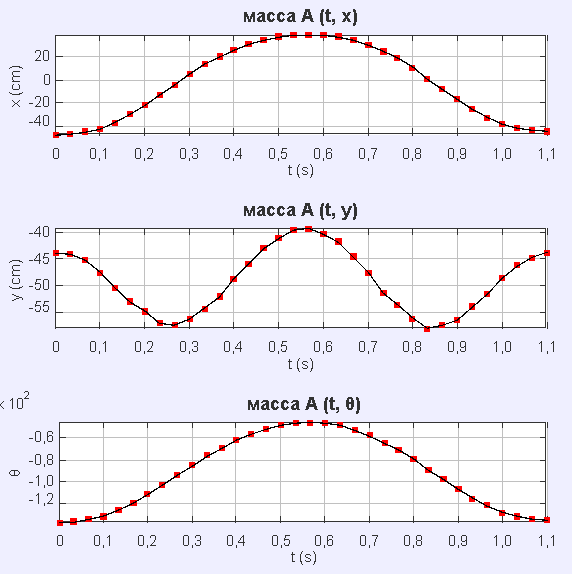
\includegraphics[width = 6cm, height = 7cm]{graph45.png}	
	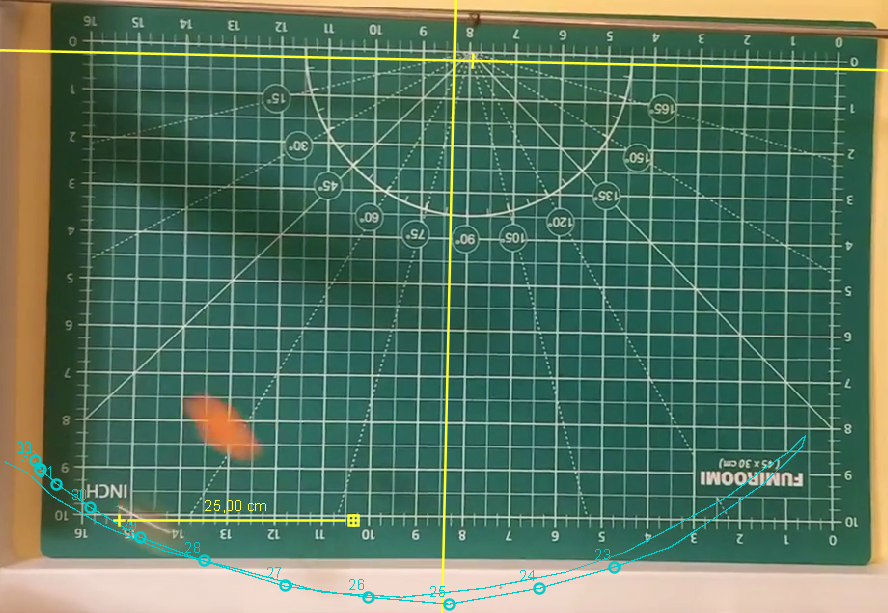
\includegraphics[width = 6.5cm, height = 5cm]{trajectory45.png}
	
	\newpage
	
	Опыт №2\\
	\(\theta_0 = 30^\circ\) градусов.\\
	Период \(T=1.03\)с.\\
	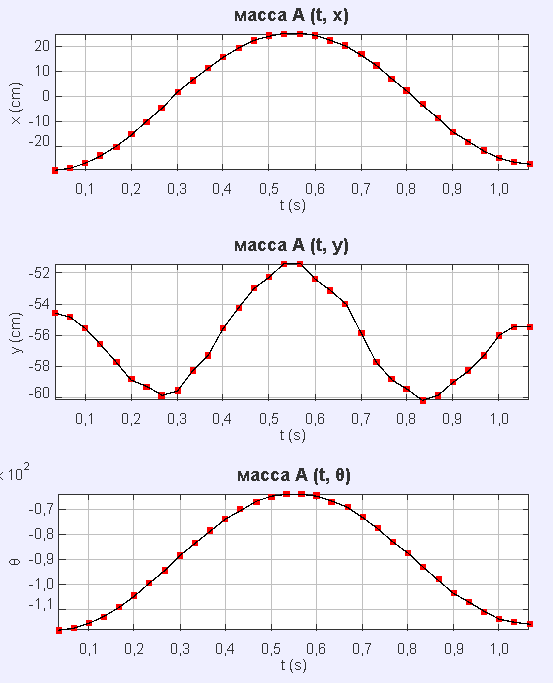
\includegraphics[width = 6cm, height = 7cm]{graph30.png}
	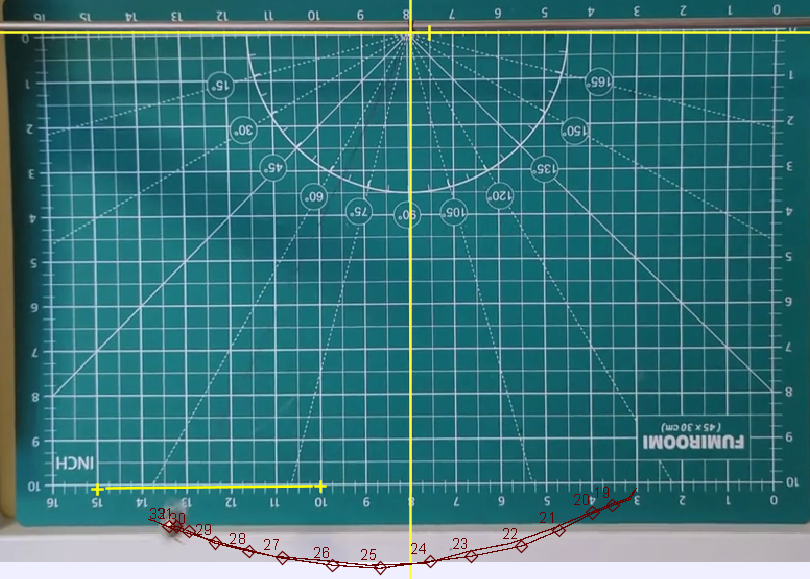
\includegraphics[width = 6.5cm, height = 5cm]{trajectory30.png}
	
	\newpage
	
	Опыт №3\\
	\(\theta_0 = 20^\circ\) градусов.\\
	Период \(T=1.00\)с.\\
	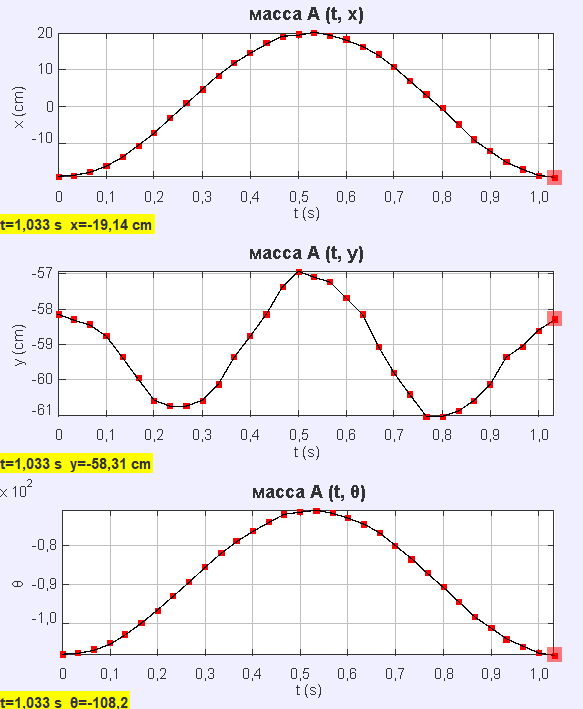
\includegraphics[width = 6cm, height = 7cm]{graph20.png}
	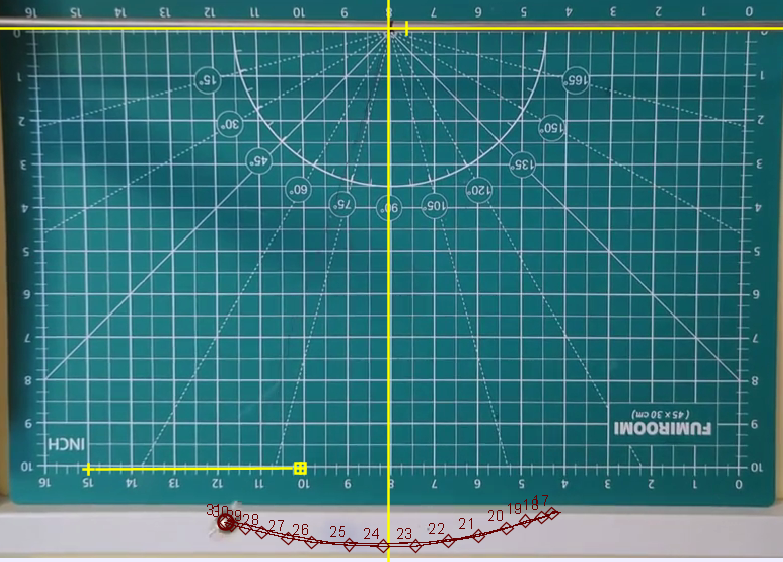
\includegraphics[width = 6.5cm, height = 5cm]{trajectory20.png}
	
	
	\newpage
	
	\large \textbf{\textcolor{structure.fg}{Отличие теории от практики}}\\
	
	формула (5)
	\[T=\frac{2\sqrt{2}}{\omega}\int\limits_0^{\theta_0}{\frac{d\theta}{\sqrt{\cos{\theta}-\cos{\theta_0}}}}.\]
	
	$\bullet$Для подсчета этого \textcolor{blue}{несобственного интеграла} пришлось адаптировать написанную для индивидуальной части программу расчета определённого интеграла\\
	$\bullet$\textcolor{blue}{Результат расчёта}: $R \approx 1.01060$с.
	\newpage

Опыт №1\\
\(T_{\text{прак}}=1.10\).\\
\(T_{\text{теор}}=\frac{2\sqrt{2}}{6.26418}\int\limits_0^{\pi/4}{\frac{d\theta}{\sqrt{\cos{\theta}-0.707106}}}=1.043573\)\\

Опыт №2\\
\(T_{\text{прак}}=1.03\).\\
\(T_{\text{теор}}=\frac{2\sqrt{2}}{6.26418}\int\limits_0^{\pi/6}{\frac{d\theta}{\sqrt{\cos{\theta}-0.866025}}}=1.020415\)\\

Опыт №3\\
\(T_{\text{прак}}=1.00\).\\
\(T_{\text{теор}}=\frac{2\sqrt{2}}{6.26418}\int\limits_0^{\pi/7.2}{\frac{d\theta}{\sqrt{\cos{\theta}-0.906307}}}=1.0150\)\\
	\newpage
	
	\large \textbf{\textcolor{structure.fg}{Доказательство (6)}}\\
	
	Требуется доказать, что
	\[\int\limits_0^{\theta_0}\frac{d\theta}{\sqrt{\cos{\theta}-\cos{\theta_0}}}=\sqrt{2}F\left(\frac{\pi}{2}, \sin{\frac{\theta_0}{2}}\right)\]
	
	Доказательство:
	
	1. Используем тригонометрическое тождество(\(\cos{x}=1-2\sin^2{\frac{\theta}{2}}\)).
	
	\[\cos{\theta}-\cos{\theta_0}=2\left(\sin^2{\frac{\theta_0}{2}}-\sin^2{\frac{\theta}{2}}\right)\]
	
	2. Подставляем интеграл.
	\[I=\int\limits_0^{\theta_0}\frac{d\theta}{\sqrt{2(\sin^2\frac{\theta_0}{2}-\sin^2\frac{\theta}{2})}}\]
	\newpage
	3. Замена переменной.\\
	Пусть \(\sin\frac{\theta}{2}=k\sin{\varphi}\), где \(k=\sin\frac{\theta_0}{2}\).\\
	При \(\theta=0: \sin{0}=k\sin\varphi\Rightarrow\varphi=0\).\\
	При \(\theta=\theta_0: \sin{\frac{\theta_0}{2}}=k\sin\varphi\Rightarrow\sin\varphi=1\Rightarrow\varphi=\frac{\pi}{2}\).\\
	
	Дифференцируем замену:\\
	\[\frac{1}{2}\cos\frac{\theta}{2}d\theta=k\cos\varphi\ d\varphi\]
	
	Выражаем \(d\theta\):\\
	\[d\theta=\frac{2k\cos\varphi}{\cos\frac{\theta}{2}}d\varphi\]
	
	\(\cos\frac{\theta}{2}=\sqrt{1-\sin^2\frac{\theta}{2}}=\sqrt{1-k^2\sin^2\varphi}\), следовательно:
	\[d\theta=\frac{2k\cos\varphi}{\sqrt{1-k^2\sin^2\varphi}}d\varphi\]
	\newpage
	
	4. Знаменатель исходного интеграла:
	\[\sqrt{2(k^2-k^2sin^2\varphi)}=\sqrt{2k^2(1-sin^2\varphi)}=\sqrt{2}k \cos\varphi\]
	
	5. Подставляем все в интеграл:
	\[I=\int\limits_0^{\pi/2}\frac{\frac{2k \cos\varphi}{\sqrt{1-k^2\sin^2\varphi}}d\varphi}{\sqrt{2}k \cos\varphi}=\sqrt{2}\int\limits_0^{\pi/2}\frac{d\varphi}{\sqrt{1-k^2sin^2\varphi}}\]
	
	Таким образом \[I=\sqrt{2}F\left(\frac{\pi}{2},\sin\frac{\theta_0}{2}\right)\]
	
	\newpage
	
	\large \textbf{\textcolor{structure.fg}{Эллиптический интеграл}}\\
	
	\[K(k)=\int\limits_0^{\pi/2}\frac{du}{\sqrt{1-k^2\sin^2{u}}}=
	\frac{\pi}{2}\sum\limits_{n=0}^{\infty}\left(\frac{(2n-1)!!}{(2n)!!}k^n\right)^2\]
	
	Для \(n=0\):\\
	\(\left(\frac{(2n-1)!!}{(2n)!!}k^n\right)^2=\left(\frac{(-1)!!}{(0)!!}\right)^2=1^2=1\)\\
	
	Для \(n=1\):\\
	\(\left(\frac{(2n-1)!!}{(2n)!!}k^n\right)^2=
	\left(\frac{(1)!!}{(2)!!}k\right)^2=\left(\frac{1}{2}k\right)^2=\frac{k^2}{4}\)\\
	
	Для \(n=2\):\\
	\(\left(\frac{(2n-1)!!}{(2n)!!}k^n\right)^2=
	\left(\frac{(3)!!}{(4)!!}k^2\right)^2=
	\left(\frac{1 \cdot 3}{2 \cdot 4}k^2\right)^2=\frac{9k^4}{64}\)\\
	
	Значит при \(n=2\):\\
	\[K(k)=\frac{\pi}{2}\left(1+\frac{k^2}{4}+\frac{9k^4}{64}\right)\]
	
	\newpage
	
	Воспользуемся эллептическим интегралом для расчета периода колебаний маятника при большой амплитуде по формуле:
	
	\[T=\frac{4}{\omega _{0}}K\left(\sin \frac{\theta _{0}}{2}\right)\]
	Рассмотрим \(\theta_0 = 30^{\circ}, \sin{\frac{\theta_0}{2}=0.2588}\) для примера с нашим маятником. Тогда 
	
	\textcolor{orange}{При \(n=0\):}\\
	\(T=\frac{4}{6.26418}K\left(\sin \frac{\theta_{0}}{2}\right)=
	0.638551 \cdot \frac{\pi}{2}=1.00302\)\\[0.5cm]
	
	\textcolor{orange}{При \(n=1\):}\\
	\(T=\frac{4}{6.26418}K\left(\sin \frac{\theta_{0}}{2}\right)=
	0.638551 \cdot \frac{\pi}{2}(1+\frac{\sin^2{\frac{\theta_0}{2}}}{4})=
	1.00302 \cdot (1+\frac{0.2588^2}{4})=1.00302 \cdot 1.016746 = 1.0198165\)\\[0.5cm]
	
	\textcolor{orange}{При \(n=2\):}\\
	\(T=\frac{4}{6.26418}K\left(\sin \frac{\theta_{0}}{2}\right)=
	0.638551 \cdot \frac{\pi}{2}(1+\frac{\sin^2{(15^\circ)}}{4}+\frac{9\sin^4{(15^\circ)}}{64})=
	1.00302 \cdot (1+\frac{0.2588^2}{4}+\frac{0.2588^4}{64})=
	1.00302 \cdot (1 + 0.016746 + 0.000070) = 1.0198868\)\\
	
	\newpage
	
	\large \textbf{\textcolor{structure.fg}{Оценка погрешностей и выводы}}\\
	Во время проведения эксперимента источником погрешности были:
	\begin{itemize}
		\item Неточность измерения длины L.
		\item Неточность определения угла \(\theta_0\).
		\item Сопротивление воздуха, трение в подвесе.
		\item Малая частота кадров, плохое качество видео.
	\end{itemize}
	А во время вычислений:
	\begin{itemize}
		\item Погрешность компьютерных вычислений.
		\item Погрешность от использования конечного числа членов ряда (7).
	\end{itemize}
	\textbf{Выводы}:
	
	Нелинейная модель точнее описывает движение при больших амплитудах.
	
	Ряд (7) позволяет удобно вычислять период без численного интегрирования, но при больших углах требует многих членов.
	
\end{document}